% Options for packages loaded elsewhere
% Options for packages loaded elsewhere
\PassOptionsToPackage{unicode}{hyperref}
\PassOptionsToPackage{hyphens}{url}
%


\PassOptionsToPackage{table}{xcolor}

\documentclass[
  10pt,
  letterpaper,
]{article}
\usepackage{xcolor}
\usepackage[top=0.85in,left=2.75in,footskip=0.75in]{geometry}
\usepackage{amsmath,amssymb}
\setcounter{secnumdepth}{-\maxdimen} % remove section numbering
\usepackage{iftex}
\ifPDFTeX
  \usepackage[T1]{fontenc}
  \usepackage[utf8]{inputenc}
  \usepackage{textcomp} % provide euro and other symbols
\else % if luatex or xetex
  \usepackage{unicode-math} % this also loads fontspec
  \defaultfontfeatures{Scale=MatchLowercase}
  \defaultfontfeatures[\rmfamily]{Ligatures=TeX,Scale=1}
\fi
\usepackage{lmodern}
\ifPDFTeX\else
  % xetex/luatex font selection
\fi
% Use upquote if available, for straight quotes in verbatim environments
\IfFileExists{upquote.sty}{\usepackage{upquote}}{}
\IfFileExists{microtype.sty}{% use microtype if available
  \usepackage[]{microtype}
  \UseMicrotypeSet[protrusion]{basicmath} % disable protrusion for tt fonts
}{}
\makeatletter
\@ifundefined{KOMAClassName}{% if non-KOMA class
  \IfFileExists{parskip.sty}{%
    \usepackage{parskip}
  }{% else
    \setlength{\parindent}{0pt}
    \setlength{\parskip}{6pt plus 2pt minus 1pt}}
}{% if KOMA class
  \KOMAoptions{parskip=half}}
\makeatother


\usepackage{longtable,booktabs,array}
\newcounter{none} % for unnumbered tables
\usepackage{calc} % for calculating minipage widths
% Correct order of tables after \paragraph or \subparagraph
\usepackage{etoolbox}
\makeatletter
\patchcmd\longtable{\par}{\if@noskipsec\mbox{}\fi\par}{}{}
\makeatother
% Allow footnotes in longtable head/foot
\IfFileExists{footnotehyper.sty}{\usepackage{footnotehyper}}{\usepackage{footnote}}
\makesavenoteenv{longtable}
\usepackage{graphicx}
\makeatletter
\newsavebox\pandoc@box
\newcommand*\pandocbounded[1]{% scales image to fit in text height/width
  \sbox\pandoc@box{#1}%
  \Gscale@div\@tempa{\textheight}{\dimexpr\ht\pandoc@box+\dp\pandoc@box\relax}%
  \Gscale@div\@tempb{\linewidth}{\wd\pandoc@box}%
  \ifdim\@tempb\p@<\@tempa\p@\let\@tempa\@tempb\fi% select the smaller of both
  \ifdim\@tempa\p@<\p@\scalebox{\@tempa}{\usebox\pandoc@box}%
  \else\usebox{\pandoc@box}%
  \fi%
}
% Set default figure placement to htbp
\def\fps@figure{htbp}
\makeatother





\setlength{\emergencystretch}{3em} % prevent overfull lines

\providecommand{\tightlist}{%
  \setlength{\itemsep}{0pt}\setlength{\parskip}{0pt}}



 
\usepackage[numbers,square,comma]{natbib}
\bibliographystyle{plos2015}


% Use adjustwidth environment to exceed column width (see example table in text)
\usepackage{changepage}

% marvosym package for additional characters
\usepackage{marvosym}

% cite package, to clean up citations in the main text. Do not remove.
% Using natbib instead
% \usepackage{cite}

% Use nameref to cite supporting information files (see Supporting Information section for more info)
\usepackage{nameref,hyperref}

% line numbers
\usepackage[right]{lineno}

% ligatures disabled
\usepackage{microtype}
\DisableLigatures[f]{encoding = *, family = * }

% create "+" rule type for thick vertical lines
\newcolumntype{+}{!{\vrule width 2pt}}

% create \thickcline for thick horizontal lines of variable length
\newlength\savedwidth
\newcommand\thickcline[1]{%
  \noalign{\global\savedwidth\arrayrulewidth\global\arrayrulewidth 2pt}%
  \cline{#1}%
  \noalign{\vskip\arrayrulewidth}%
  \noalign{\global\arrayrulewidth\savedwidth}%
}

% \thickhline command for thick horizontal lines that span the table
\newcommand\thickhline{\noalign{\global\savedwidth\arrayrulewidth\global\arrayrulewidth 2pt}%
\hline
\noalign{\global\arrayrulewidth\savedwidth}}

% Text layout
\raggedright
\setlength{\parindent}{0.5cm}
\textwidth 5.25in 
\textheight 8.75in

% Bold the 'Figure #' in the caption and separate it from the title/caption with a period
% Captions will be left justified
\usepackage[aboveskip=1pt,labelfont=bf,labelsep=period,justification=raggedright,singlelinecheck=off]{caption}
\renewcommand{\figurename}{Fig}

% Remove brackets from numbering in List of References
\makeatletter
\renewcommand{\@biblabel}[1]{\quad#1.}
\makeatother

% Header and Footer with logo
\usepackage{lastpage,fancyhdr}
\usepackage{epstopdf}
%\pagestyle{myheadings}
\pagestyle{fancy}
\fancyhf{}
%\setlength{\headheight}{27.023pt}
%\lhead{\includegraphics[width=2.0in]{PLOS-submission.eps}}
\rfoot{\thepage/\pageref{LastPage}}
\renewcommand{\headrulewidth}{0pt}
\renewcommand{\footrule}{\hrule height 2pt \vspace{2mm}}
\fancyheadoffset[L]{2.25in}
\fancyfootoffset[L]{2.25in}
\lfoot{\today}
\usepackage{booktabs}
\usepackage{longtable}
\usepackage{array}
\usepackage{multirow}
\usepackage{wrapfig}
\usepackage{float}
\usepackage{colortbl}
\usepackage{pdflscape}
\usepackage{tabularx}
\usepackage{xltabular}
\usepackage{threeparttable}
\usepackage{threeparttablex}
\usepackage[normalem]{ulem}
\usepackage{makecell}
\usepackage{xcolor}
\setlength{\parindent}{0pt}
\makeatletter
\@ifpackageloaded{caption}{}{\usepackage{caption}}
\AtBeginDocument{%
\ifdefined\contentsname
  \renewcommand*\contentsname{Table of contents}
\else
  \newcommand\contentsname{Table of contents}
\fi
\ifdefined\listfigurename
  \renewcommand*\listfigurename{List of Figures}
\else
  \newcommand\listfigurename{List of Figures}
\fi
\ifdefined\listtablename
  \renewcommand*\listtablename{List of Tables}
\else
  \newcommand\listtablename{List of Tables}
\fi
\ifdefined\figurename
  \renewcommand*\figurename{Figure}
\else
  \newcommand\figurename{Figure}
\fi
\ifdefined\tablename
  \renewcommand*\tablename{Table}
\else
  \newcommand\tablename{Table}
\fi
}
\@ifpackageloaded{float}{}{\usepackage{float}}
\floatstyle{ruled}
\@ifundefined{c@chapter}{\newfloat{codelisting}{h}{lop}}{\newfloat{codelisting}{h}{lop}[chapter]}
\floatname{codelisting}{Listing}
\newcommand*\listoflistings{\listof{codelisting}{List of Listings}}
\makeatother
\makeatletter
\makeatother
\makeatletter
\@ifpackageloaded{caption}{}{\usepackage{caption}}
\@ifpackageloaded{subcaption}{}{\usepackage{subcaption}}
\makeatother
\usepackage{bookmark}
\IfFileExists{xurl.sty}{\usepackage{xurl}}{} % add URL line breaks if available
\urlstyle{same}
\hypersetup{
  pdftitle={Disentangling the drivers of heterogeneity in SARS-CoV-2 transmission from data on viral load and daily contact rates},
  pdfauthor={Billy J Quilty; Lloyd AC Chapman; James D Munday; Kerry LM Wong; Amy Gimma; Suzanne Pickering; Stuart JD Neil; Rui Pedro Galao; W John Edmunds; Christopher I Jarvis; Adam J Kucharski},
  hidelinks,
  pdfcreator={LaTeX via pandoc}}




\begin{document}
\vspace*{0.2in}

% Title must be 250 characters or less.
\begin{flushleft}
{\Large
\textbf\newline{Disentangling the drivers of heterogeneity in SARS-CoV-2
transmission from data on viral load and daily contact
rates} % Please use "sentence case" for title and headings (capitalize only the first word in a title (or heading), the first word in a subtitle (or subheading), and any proper nouns).
}
\newline
\\
% Insert author names, affiliations and corresponding author email (do not include titles, positions, or degrees).
Billy J Quilty\textsuperscript{1,2\Yinyang}, Lloyd AC
Chapman\textsuperscript{1,3\Yinyang*}, James D
Munday\textsuperscript{1,5}, Kerry LM Wong\textsuperscript{1}, Amy
Gimma\textsuperscript{1}, Suzanne Pickering\textsuperscript{4}, Stuart
JD Neil\textsuperscript{4}, Rui Pedro Galao\textsuperscript{4}, W John
Edmunds\textsuperscript{1}, Christopher I
Jarvis\textsuperscript{1}, Adam J Kucharski\textsuperscript{1}
\\
\bigskip
\textbf{1} Centre for Mathematical Modelling of Infectious Diseases,
London School of Hygiene and Tropical Medicine, \\ \textbf{2} Center for
Global Health, Charite Universitatsmedizin Berlin, \\ \textbf{3} School
of Mathematical Sciences, Lancaster University, \\ \textbf{4} Department
of Infectious Diseases, School of Immunology and Microbial Sciences,
King's College London, \\ \textbf{5} Department of Biosystems Science
and Engineering, ETH Zurich, Basel, 
\bigskip

% Insert additional author notes using the symbols described below. Insert symbol callouts after author names as necessary.
% 
% Remove or comment out the author notes below if they aren't used.
%
% Primary Equal Contribution Note
\Yinyang These authors contributed equally to this work.

% Additional Equal Contribution Note
% Also use this double-dagger symbol for special authorship notes, such as senior authorship.
%\ddag These authors also contributed equally to this work.

% Current address notes

% Deceased author note

% Group/Consortium Author Note

% Use the asterisk to denote corresponding authorship and provide email address in note below.
* l.chapman4@lancaster.ac.uk

\end{flushleft}

\section*{Abstract}
SARS-CoV-2 transmission is highly overdispersed, with a minority of
individuals responsible for the majority of transmission, though the
drivers of this heterogeneity are unclear. Here, we assess the
contribution of variation in viral load and daily contact rates to this
heterogeneity by combining published viral load estimates and contact
survey data in a mathematical model to estimate the secondary infection
distribution. Using data from the BBC Pandemic and CoMix contact
surveys, we estimate the secondary infection distribution throughout the
pandemic in the UK in 2020, and the effectiveness of frequent and
pre-event rapid testing for reducing superspreading events. We find that
individual heterogeneity in contacts rather than individual
heterogeneity in shedding is the main driver of observed heterogeneity
in the secondary infection distribution. Our results suggest that
everyone testing every 3 days would reduce the reproduction number below
1 and be equivalent in terms of impact on secondary infections to
everyone testing only before events with a minimum event size of 10 for
pre-pandemic contact levels. This work demonstrates the potential for
using viral load and contact data to estimate heterogeneity in
transmission and the effectiveness of rapid testing strategies for
curbing transmission in future pandemics.


\linenumbers

\subsection{Author Summary}\label{author-summary}

SARS-CoV-2 spreads mainly through superspreading, with around 20\% of
infected individuals responsible for around 80\% of secondary
infections. Previous studies have inferred this using plausible
assumptions about contact rates and viral load dynamics. Here, we
instead integrate data from real contact surveys conducted in the UK
before and during the COVID-19 pandemic with published estimates of
viral load trajectories and infectiousness to estimate the average and
variation in numbers of secondary infections per case over the first
year of the pandemic. Our results are consistent with observed
reductions in secondary infections during periods of contact
restrictions in the UK. We show that variation in numbers of daily
contacts can be used to monitor superspreading risk in real-time during
an epidemic. When combined with regular rapid testing, which identifies
individuals with high viral loads when they are most infectious, this
offers a means of effectively reducing transmission and avoiding costly
blanket interventions by targeting restrictions to when and where they
are most needed.

\subsection{Introduction}\label{introduction}

Transmission of SARS-CoV-2 occurs primarily through superspreading, with
20\% of infections generating around 80\% of secondary infections
\citep{endo2020}. A review and meta-regression by Chen et al.
\citep{chen2021} indicates that substantial variation in the respiratory
viral load of individuals infected with SARS-CoV-2 is a driver of
overdispersion in secondary infection generation. However, as most
studies cited measured viral load at one point over the course of
infection, this review could not answer whether this is due to some
individuals being more infectious than others generally
(``between-person infectiousness variability'' hypothesis) or whether
most individuals pass through a highly infectious period which happens
to coincide with a period of high contact (``between-person contact
variability and within-person infectiousness variability'' hypothesis).
High contact rates are a prerequisite for infecting a large number of
people, and hence the potential for superspreading should have varied
over the course of the COVID-19 pandemic as contact distributions
changed with the enactment and relaxation of restrictions.

In this paper, we reconstruct the secondary infection distribution of
SARS-CoV-2 using a model of intra- and inter-host heterogeneity in
infectiousness derived from published data on viral load trajectories
and infectivity combined with data on reported numbers of daily contacts
from two social contact surveys in the UK. As overdispersion in the
social contact data has not previously been analysed or reported, we
first perform a descriptive analysis of the social contact data. While
previous models of superspreading of SARS-CoV-2 have either fitted to
summary data on key epidemiological metrics, such as the mean
reproduction number and distributions of individual-level numbers of
secondary cases from contact tracing studies \citep{goyal2021}, to
estimate social contact rates, or considered a wide range of plausible
contact rates \citep{susswein2020}, here we estimate the secondary
infection distribution from first principles using data on social
contacts gathered prior to and during the pandemic in the UK. This
allows us to characterise variation in the secondary infection
distribution over time under different levels of restrictions on
contacts. We also consider the impact of rapid lateral flow antigen
tests (LFTs), which are able to detect individuals with high viral loads
when they are most likely to be infectious
\citep{killingley2022, ke2022}, taken regularly or before events on the
mean reproduction number and the potential for superspreading with
differing levels of adherence and background contact rates.

The distribution of the number of secondary infections generated by each
infectious individual \(i\), \(R_i\), can be assumed to be negative
binomial with mean equal to the mean number of secondary infections
\(R\) and overdispersion parameter \(k\) representing the variation in
the number of secondary infections, with smaller values of \(k\)
representing greater variation, \[
R_i \sim \operatorname{NegBin}(k, R)
\] such that the variance in \(R_i\) is \[
\operatorname{Var}(R_i) = R + \frac{R^2}{k}.
\] Even if the mean number of secondary infections \(R\) is below 1,
there may still be a considerable probability of one or more secondary
infections if \(k\) is small. We estimate the utility of regular rapid
LFTs on reducing \(R\) and the potential for superspreading events by
decreasing variation in numbers of secondary infections, that is,
increasing \(k\).

\subsection{Methods}\label{methods}

\subsubsection{Ethics}\label{ethics}

This study only involved secondary analysis of publicly available
contact survey data and SARS-CoV-2 viral load data. Secondary analysis
of these data was approved by the London School of Hygiene and Tropical
Medicine Observational Research Ethics Committee (ref 14400 and ref
21795).

\subsubsection{Contact data}\label{contact-data}

\paragraph{BBC Pandemic survey}\label{bbc-pandemic-survey}

The BBC Pandemic contact survey was conducted between September 2017 and
December 2018 as part of a BBC Four documentary and involved over 40,000
participants (full details are published elsewhere
\citep{klepac2018, klepac2020, kucharski2020}). Participants used an app
to record their personal basic demographic information and the number of
social contacts they made during the previous 24-hour period, as well as
information such as the contact's age, type of interaction, and setting
(home, work, school, other). Children under 13 years of age were
excluded from participating for ethical reasons.

\paragraph{CoMix survey}\label{comix-survey}

The CoMix survey was a behavioural survey launched on 24th of March 2020
to gather social and behavioural data to aid the response to the
COVID-19 pandemic. The contact survey was based on the POLYMOD contact
survey \citep{mossong2008}. The sample was broadly representative of the
UK adult population. Participants were invited to respond to the survey
once every two weeks. Weekly data was collected by running two
alternating panels. Parents completed the survey on behalf of children
(17 years old or younger). Participants recorded direct, face-to-face
contacts made on the previous day, specifying certain characteristics
for each contact including the age and sex of the contact, whether
contact was physical (skin-to-skin contact), and where contact occurred
(e.g.~at home, work, while undertaking leisure activities, etc.). Full
details have been published elsewhere \citep{gimma2022}.

From the 24th May 2020 onwards, the CoMix survey included the ability to
record an estimated mass contacts count in situations where it would be
infeasible to record the detailed information of all contacts made, such
as large gatherings. Since the BBC Pandemic survey did not include this
option, and this potentially truncated the true contact distribution, we
conducted a sensitivity analysis of the effect on \(R\) and \(k\) of
imputing a heavier tail for the BBC Pandemic contact distribution. We
did this by fitting a generalised Pareto distribution to the number of
individuals reporting over 250 contacts in relaxed restrictions time
periods (``Relaxed restrictions'' and ``School reopening'' in Table 1)
from the CoMix data and sampling proportionally from this distribution
for the BBC Pandemic contacts.

\subsubsection{Analysis of social contact
data}\label{analysis-of-social-contact-data}

We compared contact distributions (overall and stratified by household
and out-of-household) for the BBC Pandemic survey
\citep{klepac2018, klepac2020, kucharski2020} and CoMix survey
\citep{jarvis2020, gimma2022}. To account for differences in numbers of
participants per time period, we calculated and plotted the percentage
of participants reporting more than 5, 10, 20, 50, 100, and 200 contacts
in the 24-hour period prior to filling in the survey for the BBC
Pandemic survey (here referred to as Pre-pandemic) and nine indicative
time periods between March 2020 and May 2021 from the CoMix survey
representing different levels of restrictions, as defined in previous
work \citep{jarvis2020, gimma2022} (Table 1). We fitted negative
binomial distributions to numbers of daily contacts in the different
time periods to estimate the mean and dispersion of the contact
distributions. To assess whether the negative binomial adequately
captured the contact distribution, or whether an excess of zero-contact
individuals required a zero-inflated extension, we additionally fitted a
zero-inflated negative binomial (ZINB) distribution to the
per-individual daily contact counts for three indicative time periods
(Pre-pandemic, 1st lockdown, School reopening) and compared models using
the Akaike information criterion (AIC) and a likelihood ratio test
(LRT). The negative binomial was found to be sufficient in all periods
(zero-inflation parameter \(\pi < 6\times 10^{-8}\), \(\Delta\)AIC =
+2.0, LRT \(p > 0.97\); Table S2).

\subsubsection{Reconstruction of secondary infection
distribution}\label{reconstruction-of-secondary-infection-distribution}

We reconstructed the secondary infection distribution of SARS-CoV-2 in
the UK over the course of 2020 as described below. We restricted our
analysis to the first six time periods of the CoMix survey in 2020 (23rd
March to 19th December) prior to the widespread emergence of more
transmissible variants and mass vaccination.

\paragraph{Viral load trajectories}\label{viral-load-trajectories}

To predict the distribution of individual-level transmission at
different points in time, we simulated 10,000 individual respiratory
viral load trajectories of index cases over the course of infection. The
viral load of each index case was constructed from a piecewise linear
function of their Ct values defined by a proliferation phase (days from
exposure to peak, \(d_p\)), a clearance phase (days from peak to
cessation, \(d_r\)) and a peak Ct value, \(\mathrm{Ct}_p\). The three
parameters were drawn from distributions given in Kissler et al.
\citep{kissler2021} (Figure~\ref{fig-diagram}): \[
\begin{aligned}
d_p &\sim N_{[1,14]}(2.0, 13.4), \\
\mathrm{Ct}_p &\sim N_{[0,40]}(20.2, 19.5), \\
d_r &\sim N_{[1,30]}(6.3, 6.8)
\end{aligned}
\] where \(N_{[a,b]}(\mu, \sigma^2)\) denotes a truncated normal
distribution with mean \(\mu\) and variance \(\sigma^2\), and lower and
upper limits \(a\) and \(b\). The Ct value at exposure and cessation of
shedding was assumed to be 40 (negative).

The Ct value was converted to viral load \(\mathrm{vl}\) (in log10 RNA
copies/ml) via the following formula \citep{kissler2021}: \[
\mathrm{vl} = \frac{\mathrm{Ct} - b_{\mathrm{conv}}}{m_{\mathrm{conv}}} + \log_{10}(250)
\] where \(m_{\mathrm{conv}}=-3.60971\) and
\(b_{\mathrm{conv}}=40.93733\) are the slope and intercept of a linear
regression of Ct value on log10-transformed RNA concentration from a
standard curve.

\paragraph{Infectiousness}\label{infectiousness}

The probability of infectiousness for a given viral load (in Ct) was
estimated by fitting a logistic regression model to the probability of
culturing virus at that viral load \citep{pickering2021}
(Figure~\ref{fig-vl}B), \(p_{\mathrm{culture}}\): \[
\begin{aligned}
\mathrm{culture} &\sim \operatorname{Bernoulli}(p_{\mathrm{culture}}) \\
\operatorname{logit}(p_{\mathrm{culture}}) &= \beta_0 + \beta_1\,\mathrm{vl}
\end{aligned}
\] where culture is the binary outcome of whether or not virus was
cultured. The probability of infectiousness over the course of each
individual's viral load trajectory was then calculated using the
estimated regression coefficients \(\beta_0\) and \(\beta_1\) to produce
infectiousness trajectories (Figure~\ref{fig-vl}C). Uncertainty in
\(\beta_0\) and \(\beta_1\) was accounted for by drawing values for each
individual from a bivariate normal distribution centred at the maximum
likelihood estimate
\(\hat{\beta} = (\hat{\beta}_0, \hat{\beta}_1) = (-14.8, 2.1)\): \[
\boldsymbol{\beta} \sim \mathcal{N}(\hat{\boldsymbol{\beta}}, \Sigma)
\] where \(\Sigma\) is the estimated covariance matrix from the logistic
regression. Drawing values for the regression coefficients in this way
may be taken to represent a degree of variation in infectiousness
between individuals for the same viral load, as Ke et al. \citep{ke2022}
concluded was necessary to explain observed heterogeneity in
infectiousness. We use viral culture positivity as our proxy for
infectiousness because it indicates the presence of
replication-competent virus and is therefore believed to provide a
better indicator of transmission potential than Ct values from PCR
measurements \citep{drain2023}. It also allows us to make use of
empirical relationships linking viral load, viral culture positivity,
and test detection: (i) viral load determines the probability of
culturing viable virus, with the logistic relationship fitted directly
from data in Pickering et al. \citep{pickering2021}
(Figure~\ref{fig-vl}B); and (ii) LFT positivity closely tracks viable
virus in controlled human challenge studies \citep{killingley2022}.

\begin{figure}

\centering{

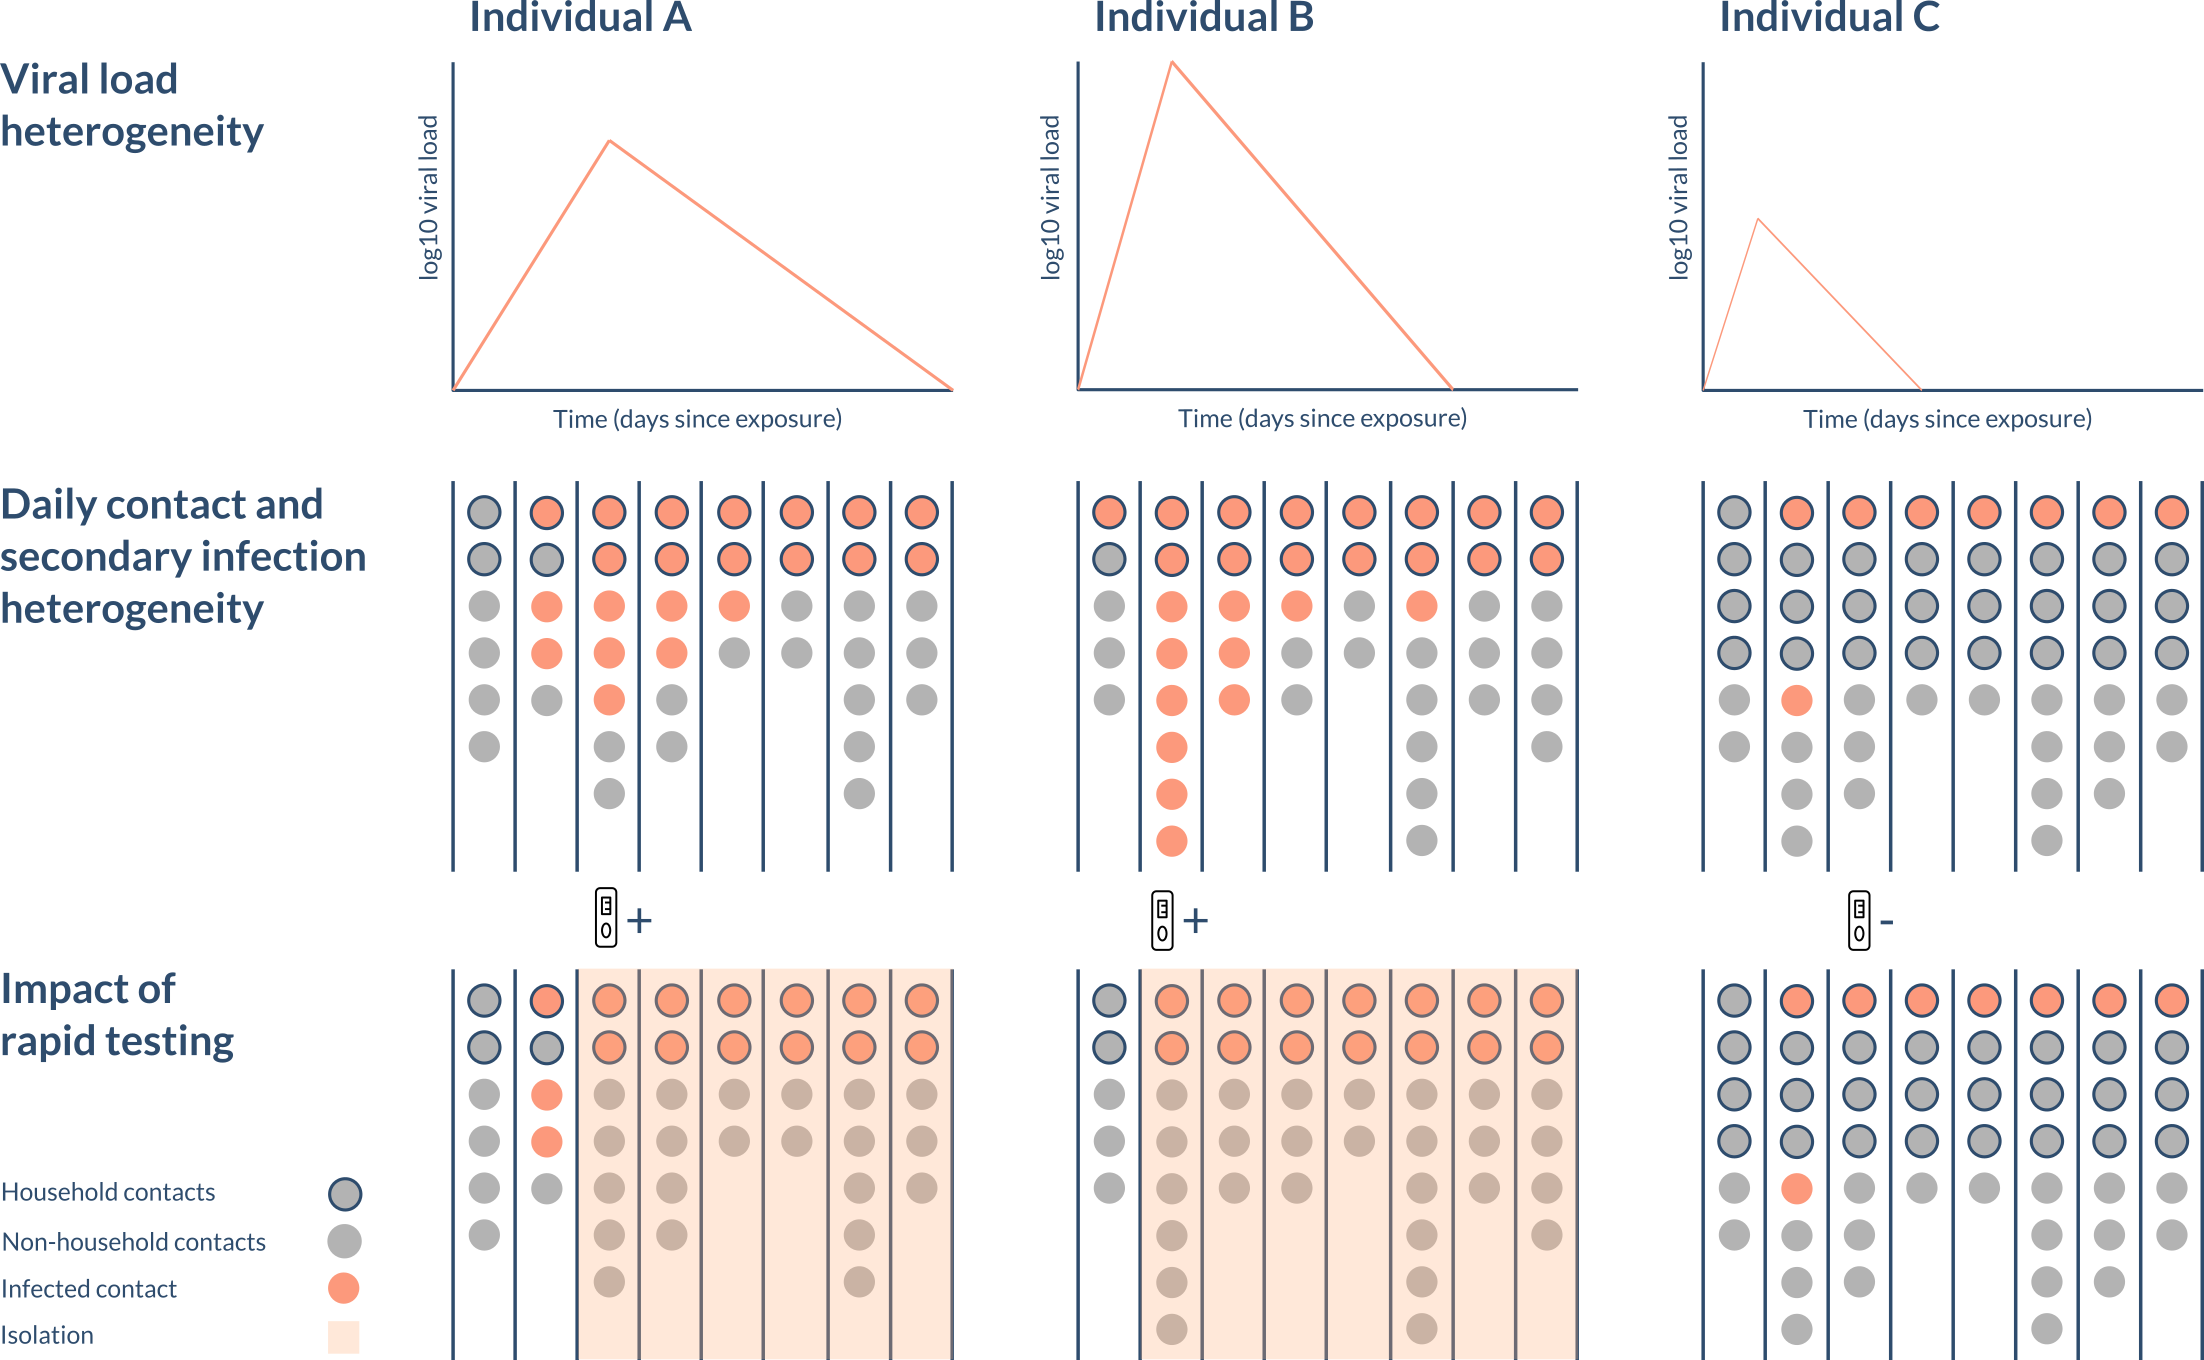
\includegraphics[width=1\linewidth,height=\textheight,keepaspectratio]{../results/manuscript_figures/fig1_diagram.png}

}

\caption{\label{fig-diagram}Schematic of the model. The viral load and
number of daily contacts (circles) varies from person to person and over
time, influencing the number of secondary infections (stratified by
household (outlined) and non-household (no outline)) they generate. The
viral load at time of testing also determines the likelihood they will
test positive and subsequently isolate.}

\end{figure}%

\paragraph{Contacts and contact
durations}\label{contacts-and-contact-durations}

For the pre-pandemic time period and each of the pandemic time periods,
we randomly sampled the number of household contacts
\(N_{\mathrm{HH},i}\) and daily non-household contacts
\(N_{\mathrm{NHH},i,t}\) for index case \(i\), where \(t\) is the time
since exposure, from the empirical contact distribution for that time
period from the BBC Pandemic contact survey
\citep{klepac2018, klepac2020, kucharski2020} and CoMix contact survey
\citep{jarvis2020, gimma2022}. The number of household and non-household
contacts were sampled jointly by sampling a survey participant at
random, to preserve correlation in individual-level numbers of household
and non-household contacts. The numbers of non-household contacts on
different days were sampled from the repeat survey responses of the
chosen participant for the given time period, to maintain correlation in
individual-level numbers of non-household contacts over time. Each
household and non-household contact had a duration,
\(\mathrm{dur}_{\mathrm{HH},i,j,t}\) and
\(\mathrm{dur}_{\mathrm{NHH},i,j,t}\), defined as the proportion of a
24-hour period that the contact lasted (Figure S1). For the pandemic
time periods the duration was sampled from the contact durations for the
same survey participant as the contact numbers, where these were
available. This ensured that correlation between number of contacts and
contact duration was maintained (Figure S2). For the pre-pandemic time
period, the duration was sampled from the contact durations in the
POLYMOD survey, as contact duration data is not publicly available for
the BBC Pandemic survey. Where the contact duration was missing, it was
randomly sampled from the pre-pandemic or pandemic contact duration
distribution according to whether it was a pre-pandemic or pandemic
contact.

\paragraph{Infections}\label{infections}

The infection process for contact between index case \(i\) and their
contact \(j\) was modelled as Bernoulli for both household and
non-household infections \[
\begin{aligned}
\mathrm{inf}_{\mathrm{HH},i,j,t} &\sim \operatorname{Bernoulli}(p_{\mathrm{HH},i,j,t}) \\
\mathrm{inf}_{\mathrm{NHH},i,j,t} &\sim \operatorname{Bernoulli}(p_{\mathrm{NHH},i,j,t})
\end{aligned}
\] with the probability of \(i\) infecting \(j\) on day \(t\) in
location \(\mathrm{X}\), \(p_{\mathrm{X},i,j,t}\), where
\(\mathrm{X} \in \{\mathrm{HH}, \mathrm{NHH}\}\), given by \[
p_{\mathrm{X},i,j,t} = 1 - \exp\left(-\beta\, p_{\mathrm{culture},i,t}\, \mathrm{dur}_{\mathrm{X},i,j,t}\right)
\] where \(\beta\) is a scaling parameter which converts the product of
the relative infectiousness of \(i\) on the day of contact,
\(p_{\mathrm{culture},i,t}\), and the duration of contact,
\(\mathrm{dur}_{\mathrm{X},i,j,t}\), into a transmission rate. This
process was iterated over each day of the index case's infection up to a
maximum infection duration of 44 days in the baseline analysis. While we
modelled infection events for household members on each day of the index
case's infection, we only counted the first infection that occurred for
each household member. In other words, household members could only be
infected once. We assumed uniform susceptibility of individuals in the
model, which does not vary by, for example, age.

The number of secondary infections for index case \(i\) (i.e.~their
individual-level reproduction number), \(R_i\), was therefore given by:
\[
R_i = \sum_{t=1}^{T_i} \left(\sum_{j=1}^{N_{\mathrm{HH},i}} \mathrm{inf}_{\mathrm{HH},i,j,t} + \sum_{j=1}^{N_{\mathrm{NHH},i,t}} \mathrm{inf}_{\mathrm{NHH},i,j,t}\right)
\] where \(T_i\) is index case \(i\)'s duration of infection (defined as
having infection detectable by PCR). We then estimated the mean, \(R\),
and overdispersion, \(k\), of the number of secondary infections by
fitting a negative binomial distribution to the \(R_i\) values across
all index cases. 95\% percentile bootstrap confidence intervals (CIs)
for the \(R\) and \(k\) estimates were calculated by bootstrapping the
simulated numbers of secondary infections with 1000 bootstrap samples,
calculating \(R\) and \(k\) for each bootstrap sample and then finding
the 2.5 and 97.5 percentiles of the distributions of the bootstrap
estimates. We calibrated \(\beta\) such that the basic reproduction
number \(R_0\), the reproduction number for the pre-pandemic time
period, was 2.5, based on estimates from the literature
\citep{jarvis2020, davies2020, spimrtuk}, for the baseline analysis and
all sensitivity analyses varying heterogeneity in contact rates and
viral load. We obtained values of \(\beta\) between 1.1 and 4.7.

\subsubsection{Contribution of contact and viral load heterogeneity to
heterogeneity in secondary
infections}\label{contribution-of-contact-and-viral-load-heterogeneity-to-heterogeneity-in-secondary-infections}

To investigate the contribution of heterogeneity in contact rates and
heterogeneity in viral load between individuals to variation in the
secondary infection distribution, we calculated the overdispersion in
secondary infections for different combinations of ``homogeneous'' and
``heterogeneous'' contact rates and viral load trajectories. In the
``homogeneous'' cases, contacts were Poisson distributed with mean equal
to the mean daily contacts for each time period and all individuals had
the median viral load trajectory (i.e.~the trajectory with the median
proliferation and clearance durations and median peak Ct value), while
in the ``heterogeneous'' cases, contacts and viral load trajectories
were allowed to vary according to their full distributions.

We performed a sensitivity analysis with greater variation in viral load
trajectories across individuals, by doubling the standard deviations of
the distributions for the proliferation time, clearance time and peak Ct
value, to test the sensitivity of the results to the degree of viral
load heterogeneity. For this sensitivity analysis, we considered onward
transmissions up to 88 days post exposure.

\subsubsection{Simulation of
interventions}\label{simulation-of-interventions}

We assessed the hypothesis that if those with the highest viral loads
are most likely to cause superspreading events, and LFTs are most
sensitive for those with the highest viral loads, then lateral flow
testing should be able to prevent superspreading events, which we
defined as infecting over 10 contacts. We determined the probability of
testing positive on an LFT at a given viral load, \(p_{\mathrm{test}}\),
by fitting a logistic regression model to data on LFT outcomes for
isolates with different viral loads \citep{pickering2021}. Detection was
then modelled via a Bernoulli draw with this detection probability, that
is, \[
\begin{aligned}
\mathrm{test} &\sim \operatorname{Bernoulli}(p_{\mathrm{test}}) \\
\operatorname{logit}(p_{\mathrm{test}}) &= \alpha_0 + \alpha_1\,\mathrm{vl}
\end{aligned}
\] where \(\alpha_0 = -9.1\) (95\% CI: -13.3, 5.0) and
\(\alpha_1 = 1.8\) (95\% CI: 1.1, 2.6) were the estimated coefficients
from the logistic regression. We then modelled index cases testing
regularly with LFTs at different frequencies (every 1, 3, and 7 days) or
only before events of a certain size (before meeting \textgreater10,
\textgreater20, \textgreater50 others) to determine the comparative
effectiveness of rapid testing to control transmission. We assumed that
a certain proportion of individuals self-isolated at home upon first
testing positive, such that their non-household contacts were decreased
to zero after the date of the positive test, but their number of
household contacts was unchanged. The remaining individuals were assumed
to continue making contacts as normal. We varied the proportion of
individuals who self-isolated upon testing positive from 0-100\% to
model varying uptake/adherence. We assumed timing of testing was not
affected by symptom onset and intensity, as we wished to model regular
and event-triggered testing regardless of symptoms. We considered three
indicative timepoints before (BBC Pandemic, 2018) and during the
pandemic (1st lockdown (March-June 2020) and the reopening of schools
(September 2020)). We reran the analysis for regular lateral flow
testing with Poisson-distributed contacts instead of overdispersed
contacts to look at the effect of contact heterogeneity on the impact of
regular testing.

The code and data for this study can be found at
https://github.com/bquilty25/superspreading\_testing.

\subsection{Results}\label{results}

\subsubsection{Changes in the distribution of social contacts with
changes in the intensity of
restrictions}\label{changes-in-the-distribution-of-social-contacts-with-changes-in-the-intensity-of-restrictions}

The age distribution of all participants in the BBC Pandemic survey and
of the participants in each of the nine periods of the CoMix survey is
shown in Figure S3. Relative to the mid-2020 age distribution of the UK
population, children and older adults (70+ years) are under-represented
in the BBC Pandemic data. The age distribution of CoMix participants is
representative of the general population (with slight
under-representation of children \(\le\) 4 years and over-representation
of adults aged 50-69 years) and remains fairly stable across the
different time periods.

Figure~\ref{fig-contacts}A and Table 1 show the proportions of survey
participants in the UK reporting more than a certain number of contacts
(5, 10, 20, 50, 100 and 200) in the previous day over time, both
pre-pandemic (BBC Pandemic survey) and from the CoMix survey for the
nine time periods during the survey with different levels of
restrictions. The percentage of individuals reporting more than 20
contacts in a day was substantially lower during the pandemic compared
to the pre-pandemic period (when it was 13.7\%), varying from a low of
0.4\% during the first lockdown from March to June 2020 to a peak of
6.1\% in September 2020, when restrictions were most relaxed and schools
reopened. The percentage of individuals reporting over 100 and 200
contacts was lower in the pre-pandemic BBC Pandemic contact survey
compared to periods of relaxed restrictions due to differences in the
reporting of high contact events. Overall, people reporting more than
50, 100, or 200 contacts made up less than 3\% of the total CoMix survey
sample.

\begin{figure}

\centering{

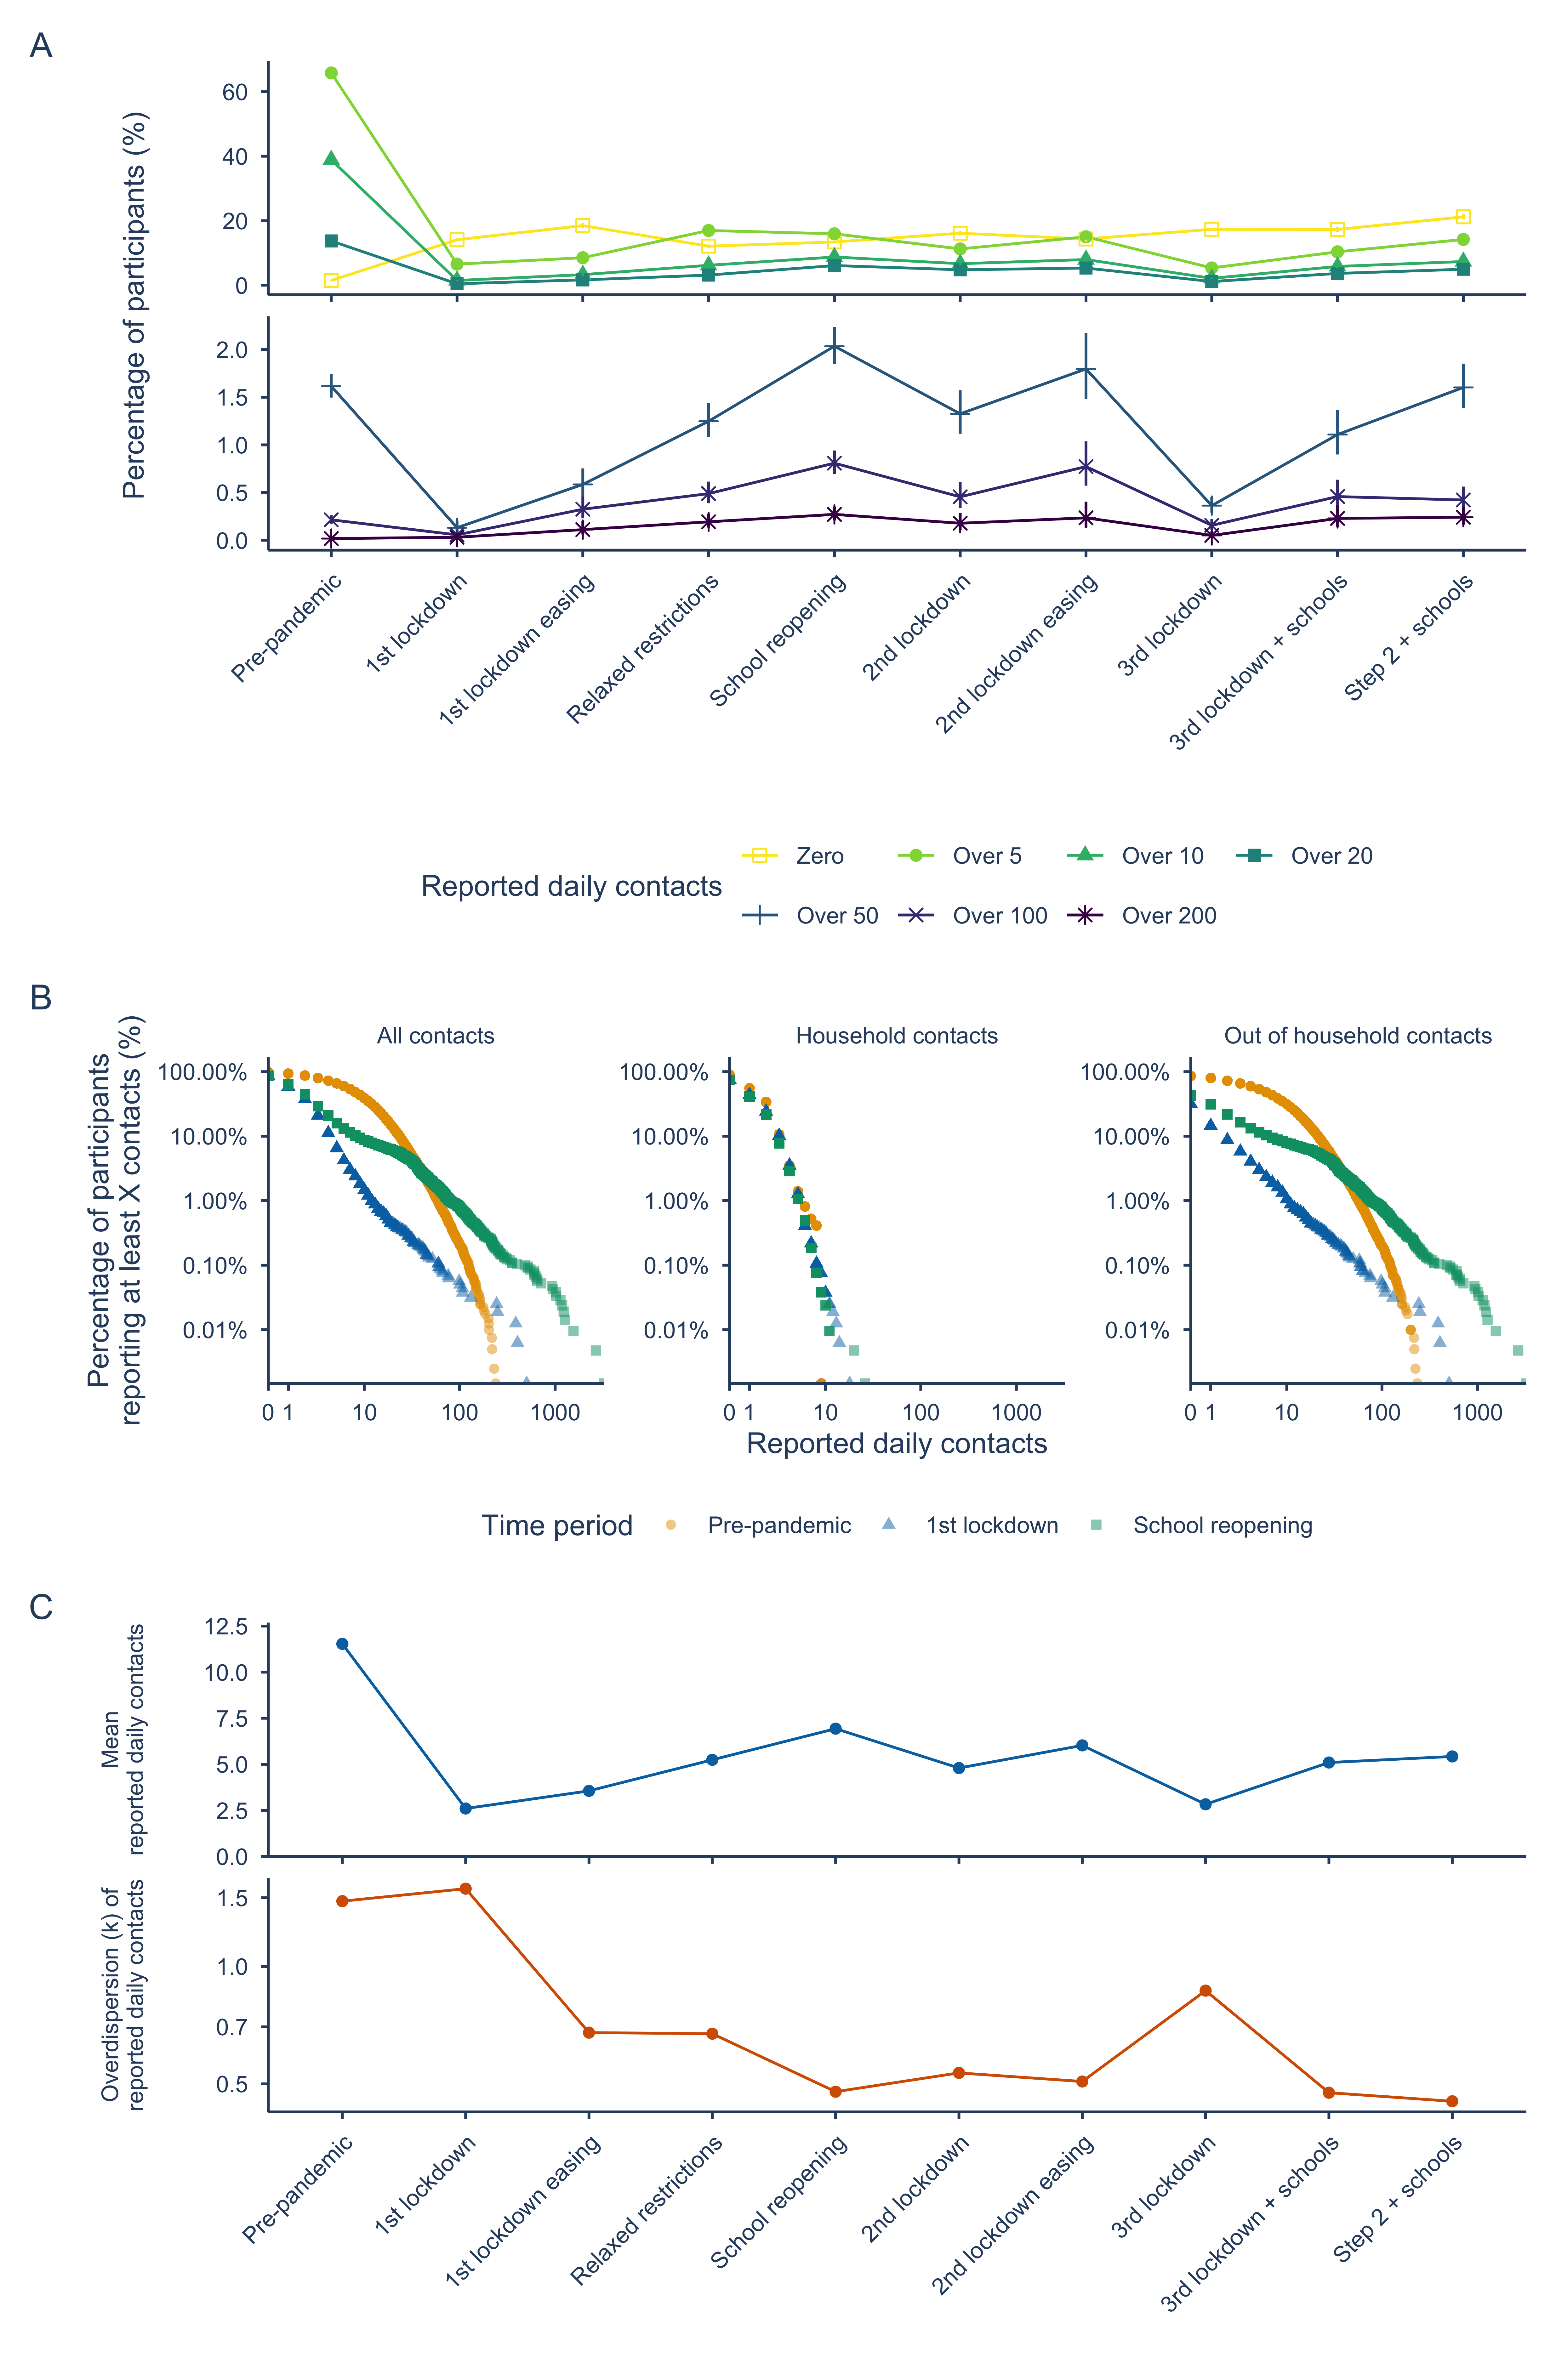
\includegraphics[width=1\linewidth,height=\textheight,keepaspectratio]{../results/manuscript_figures/fig2_contacts.png}

}

\caption{\label{fig-contacts}Changes in the distribution of social
contacts in the UK from pre-pandemic to May 2021. A. Percentage of
participants in the BBC Pandemic and CoMix contact surveys reporting
zero, over 5, 10, 20, 50, 100, and 200 daily contacts in 2018
(pre-pandemic) and nine time periods during the pandemic in the UK
between March 2020 and May 2021. Median and 95\% binomial confidence
intervals shown. B. Distribution of the number of reported daily
contacts for three indicative timepoints before and during the pandemic
in the UK in 2020. C. Mean and overdispersion parameter, \(k\), of a
negative binomial distribution fitted to contacts during the different
time periods. The heavier tail in the contact distribution for the
School reopening period in panel B compared with the Pre-pandemic period
is likely due to mass contacts not being recorded in the BBC Pandemic
contact survey, which may have truncated the contact distribution. See
Figure S4 for the BBC Pandemic contact distribution with an imputed
heavier tail, which is used to perform a sensitivity analysis.}

\end{figure}%

{

\begin{longtable}[]{@{}
  >{\raggedright\arraybackslash}p{(\linewidth - 18\tabcolsep) * \real{0.1855}}
  >{\raggedright\arraybackslash}p{(\linewidth - 18\tabcolsep) * \real{0.0887}}
  >{\raggedright\arraybackslash}p{(\linewidth - 18\tabcolsep) * \real{0.0887}}
  >{\raggedleft\arraybackslash}p{(\linewidth - 18\tabcolsep) * \real{0.0484}}
  >{\raggedleft\arraybackslash}p{(\linewidth - 18\tabcolsep) * \real{0.0887}}
  >{\raggedleft\arraybackslash}p{(\linewidth - 18\tabcolsep) * \real{0.0968}}
  >{\raggedleft\arraybackslash}p{(\linewidth - 18\tabcolsep) * \real{0.0968}}
  >{\raggedleft\arraybackslash}p{(\linewidth - 18\tabcolsep) * \real{0.0968}}
  >{\raggedleft\arraybackslash}p{(\linewidth - 18\tabcolsep) * \real{0.1048}}
  >{\raggedleft\arraybackslash}p{(\linewidth - 18\tabcolsep) * \real{0.1048}}@{}}

\caption{\label{tbl-contacts}Percentage of participants in the CoMix and
BBC Pandemic surveys with more than a certain number of contacts in
different time periods in the UK from March 2020 to May 2021, and
pre-pandemic in 2017-2018.}

\tabularnewline

\toprule\noalign{}
\begin{minipage}[b]{\linewidth}\raggedright
Time period
\end{minipage} & \begin{minipage}[b]{\linewidth}\raggedright
From
\end{minipage} & \begin{minipage}[b]{\linewidth}\raggedright
To
\end{minipage} & \begin{minipage}[b]{\linewidth}\raggedleft
N
\end{minipage} & \begin{minipage}[b]{\linewidth}\raggedleft
Over 5 (\%)
\end{minipage} & \begin{minipage}[b]{\linewidth}\raggedleft
Over 10 (\%)
\end{minipage} & \begin{minipage}[b]{\linewidth}\raggedleft
Over 20 (\%)
\end{minipage} & \begin{minipage}[b]{\linewidth}\raggedleft
Over 50 (\%)
\end{minipage} & \begin{minipage}[b]{\linewidth}\raggedleft
Over 100 (\%)
\end{minipage} & \begin{minipage}[b]{\linewidth}\raggedleft
Over 200 (\%)
\end{minipage} \\
\midrule\noalign{}
\endhead
\bottomrule\noalign{}
\endlastfoot
Pre-pandemic & 01/09/2017 & 01/12/2018 & 40162 & 65.8 & 38.9 & 13.7 &
1.6 & 0.2 & 0.0 \\
1st lockdown & 23/03/2020 & 03/06/2020 & 15971 & 6.5 & 1.5 & 0.4 & 0.1 &
0.1 & 0.0 \\
1st lockdown easing & 04/06/2020 & 29/07/2020 & 10764 & 8.5 & 3.3 & 1.6
& 0.6 & 0.3 & 0.1 \\
Relaxed restrictions & 30/07/2020 & 03/09/2020 & 15547 & 17.0 & 6.2 &
3.1 & 1.2 & 0.5 & 0.2 \\
School reopening & 04/09/2020 & 24/10/2020 & 21031 & 15.9 & 8.7 & 6.1 &
2.0 & 0.8 & 0.3 \\
2nd lockdown & 05/11/2020 & 02/12/2020 & 10106 & 11.3 & 6.7 & 4.8 & 1.3
& 0.5 & 0.2 \\
2nd lockdown easing & 03/12/2020 & 19/12/2020 & 5957 & 15.0 & 8.0 & 5.3
& 1.8 & 0.8 & 0.2 \\
3rd lockdown & 05/01/2021 & 07/03/2021 & 21755 & 5.3 & 2.1 & 1.1 & 0.4 &
0.2 & 0.1 \\
3rd lockdown + schools & 08/03/2021 & 31/03/2021 & 8300 & 10.3 & 5.8 &
3.7 & 1.1 & 0.5 & 0.2 \\
Step 2 + schools & 16/04/2021 & 16/05/2021 & 11607 & 14.2 & 7.3 & 5.0 &
1.6 & 0.4 & 0.2 \\

\end{longtable}

}

Different pandemic time periods are based on lockdowns and different
levels of restrictions.\\
\(N\) is the number of survey responses in each time period.

The estimated mean and overdispersion parameter \(k\), with lower values
indicating more overdispersion in the distribution, of numbers of daily
contacts in the UK were lower than that observed pre-pandemic, with mean
daily contacts averaging 4.7 during the pandemic compared to 11.5
pre-pandemic, and \(k\) averaging 0.7 during the pandemic compared to
1.5 pre-pandemic, indicating individuals having on average lower, but
more varied, numbers of daily contacts. These values also changed
considerably across the different periods of restrictions in a similar
pattern to the proportion of participants with high numbers of contacts,
with the mean number of daily contacts ranging from 2.6 during the first
lockdown to 6.9 when schools reopened in September 2020, with a similar
drop during the third lockdown, but less of a drop during the second
lockdown when schools remained open (Figure~\ref{fig-contacts}C). The
overdispersion in contacts, \(k\), was similar pre-pandemic and during
the first lockdown (1.5 and 1.6 respectively) then became lower,
indicating more variability, following the easing of the first lockdown,
with \(k\) between 0.5 and 0.7 in the remaining 2020 periods
(Figure~\ref{fig-contacts}C). Stratifying contacts by household and
out-of-household revealed contact rates within the household remained
stable throughout, with changing non-household contact rates driving
much of the variation in the mean and \(k\) of daily contacts over the
course of the pandemic (Figure S5). Both the mean and \(k\) of
out-of-household daily contacts remained lower than pre-pandemic contact
rates. Contact durations in CoMix differed significantly between
household and non-household contacts, with a median duration of 30
minutes (IQR: 5 -- 180 minutes) for out-of-household contacts compared
to 480 minutes (8 hours) (IQR: 180 -- 1080 minutes) for household
contacts (Figure S1). Figure S6, in which contacts are stratified by age
as well household/out-of-household, shows that both household and
out-of-household contacts in children (\textless18 years) remained
higher than those in adults throughout 2020 and early 2021, with
significant increases in out-of-household contacts of children during
periods when schools were open. Contact levels were similar for males
and females across all time periods.

\subsubsection{Variation in viral load and infectivity over the course
of
infection}\label{variation-in-viral-load-and-infectivity-over-the-course-of-infection}

Analysis by Kissler et al. \citep{kissler2021} of densely sampled viral
load trajectories in individuals infected with SARS-CoV-2 suggested
substantial variation between individuals in the duration of
proliferation and clearance phases of infection, and lowest Ct value,
inversely correlated with peak viral load (Figure~\ref{fig-vl}A).
Mapping viral load to infectivity via a logistic function based on viral
load and culture from Pickering et al. \citep{pickering2021}
(Figure~\ref{fig-vl}B), calculating the probability of infectivity by
day (Figure~\ref{fig-vl}C), then integrating under the infectivity curve
to calculate total infectious virus shed, reproduces substantial
heterogeneity in individual infectiousness as reported by Ke et al.
\citep{ke2022}. We found an 73-fold difference in individual-level
infectivity between the 2.5\% and 97.5\% percentiles of the distribution
of the area under the infectivity curve (0.08 and 5.74 arbitrary units,
respectively). Fitting a Gamma distribution to this distribution gave a
shape parameter of 1.42 (1.6 for Ke et al.). A substantial proportion
(19.4\%) of individuals were estimated to be infectious for zero days,
but the remainder were infectious for at least one day
(Figure~\ref{fig-vl}). Across all individuals, the median duration of
infectiousness around peak viral load, that is, having high enough viral
load to cause infections through culturable virus, was 2 days (95\%
prediction interval: 0, 6 days). The majority of individuals passed
through at least one day of high infectiousness (peak culture
probability greater than 0.6 for 68\% of individuals, greater than 0.8
for 53\%), and were therefore theoretically capable of causing
superspreading events given sufficient contacts of sufficient duration.
However, the percentage of infected individuals who can actually
initiate a superspreading event is much lower than 50\% because the time
window for this level of infectivity is so narrow that it must coincide
perfectly with a high number of contacts of sufficient duration for a
high number of infections to occur.

\begin{figure}

\centering{

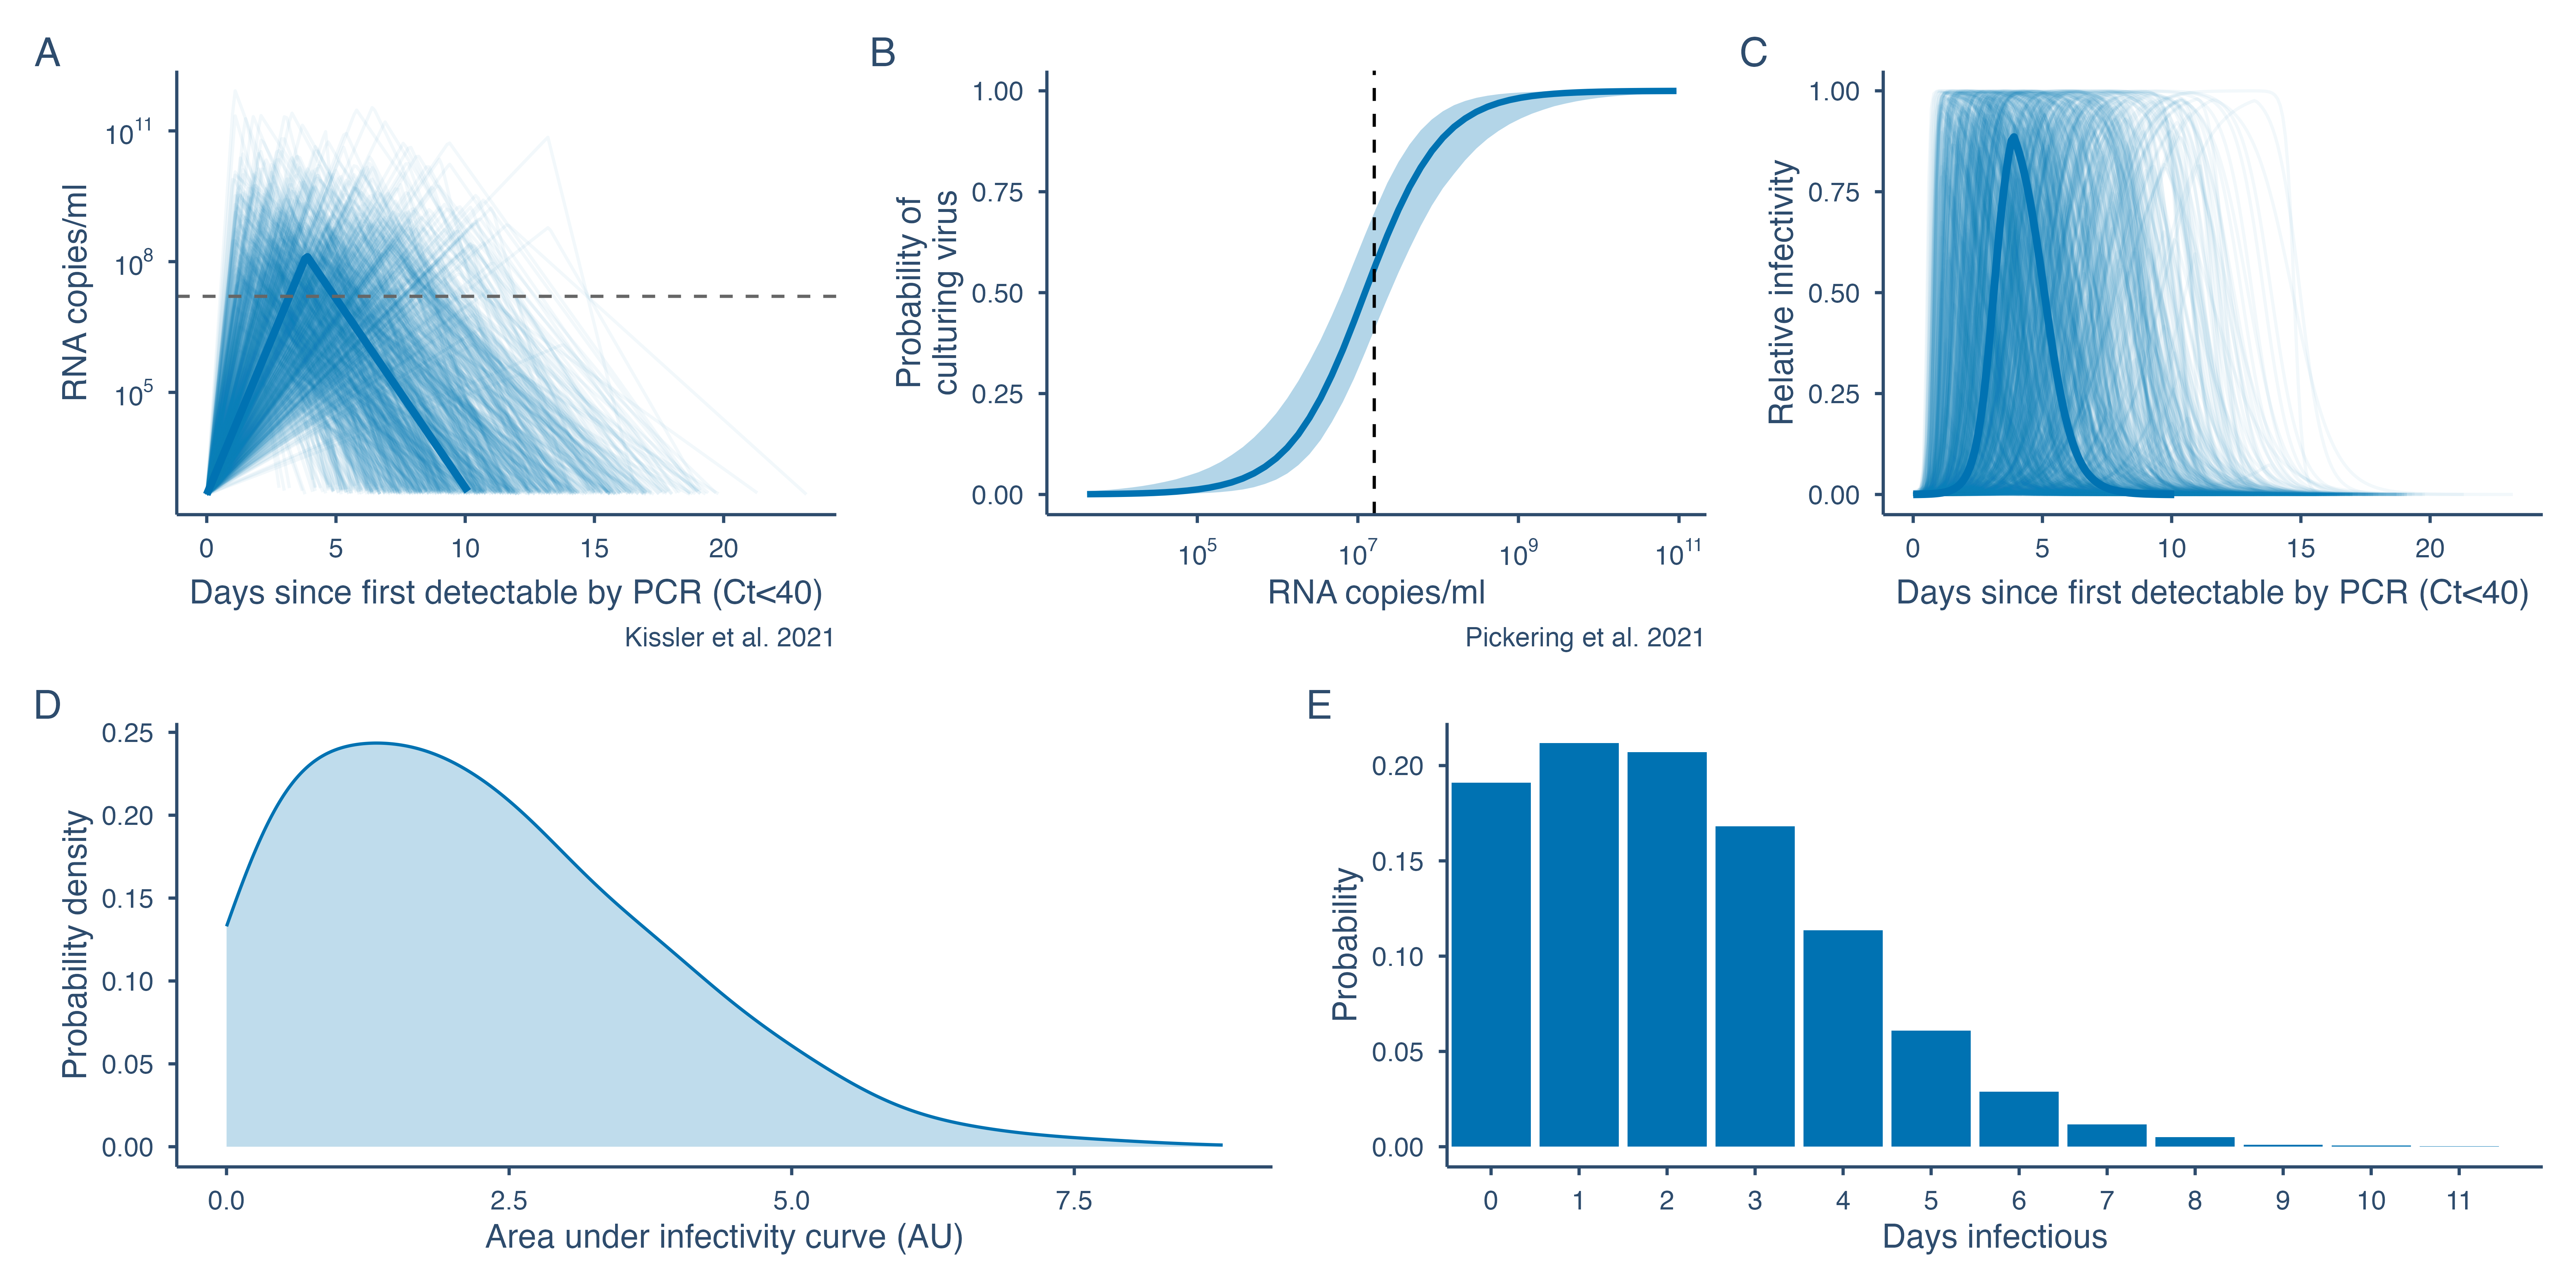
\includegraphics[width=1\linewidth,height=\textheight,keepaspectratio]{../results/manuscript_figures/fig3_vl.png}

}

\caption{\label{fig-vl}Variation in viral load progression and
infectivity. A. Individual-level viral load trajectories. B. Logistic
model for probability of culturing virus given a certain viral load. C.
Relative infectivity over time. D. Area under the infectivity curve (in
arbitrary units, AU). E. Distribution of the number of days for which
individuals were infectious. Solid lines in A and C represent median
viral load and infectivity trajectories. The dashed line in A and B
represents the RNA copies per ml required for a 50\% probability of
culturing virus or infectiousness. The shaded band in B represents the
uncertainty in the probability of culturing virus given a certain viral
load from the fitted logistic regression model from Pickering et
al.~Figure S7 shows the difference in viral load trajectories and
infectivity for the sensitivity analysis with double the standard
deviation in the viral load trajectory parameters.}

\end{figure}%

\subsubsection{Predicting transmission dynamics from heterogeneity in
contact rates and viral load
progression}\label{predicting-transmission-dynamics-from-heterogeneity-in-contact-rates-and-viral-load-progression}

Simulating secondary infections using the stochastic model described
above, we estimated the overdispersion, \(k\), in the initial secondary
infection distribution as 0.48 (95\% CI 0.47 -- 0.51)
(Figure~\ref{fig-rk}), in line with other estimates
\citep{lau2020, kremer2021}. During the first national lockdown, \(R\)
was estimated at 0.37 (95\% CI 0.35 -- 0.41) and \(k\) at 0.25 (95\% CI
0.21 -- 0.29). \(R\) rose as lockdown eased (\(R\) = 0.66, 95\% CI 0.56
-- 0.8) and restrictions were relaxed in the summer of 2020 (\(R\) = 1,
95\% CI 0.92 -- 1.1) and again as schools reopened in the autumn (\(R\)
= 1.5, 95\% CI 1.3 -- 1.6). \(R\) then decreased again during the second
lockdown to 1 (95\% CI 0.92 -- 1.2). As with contacts, \(k\) reduced as
the pandemic began, indicating more variability in the secondary
infection distribution, and varied between 0.12 and 0.17 after the first
lockdown up to the end of 2020. A sensitivity analysis imputing a
heavier tail for the BBC Pandemic contact distribution based on the
tails of contact distributions from relaxed restriction periods during
the CoMix survey led to a small increase in \(R_0\) from 2.5 (95\% CI
2.4 -- 2.6) to 2.8 (95\% CI 2.6 -- 3) and a small reduction in \(k\)
from 0.48 (95\% CI 0.46 -- 0.51) to 0.44 (95\% CI 0.4 -- 0.49) (Table
S1).

\begin{figure}

\centering{

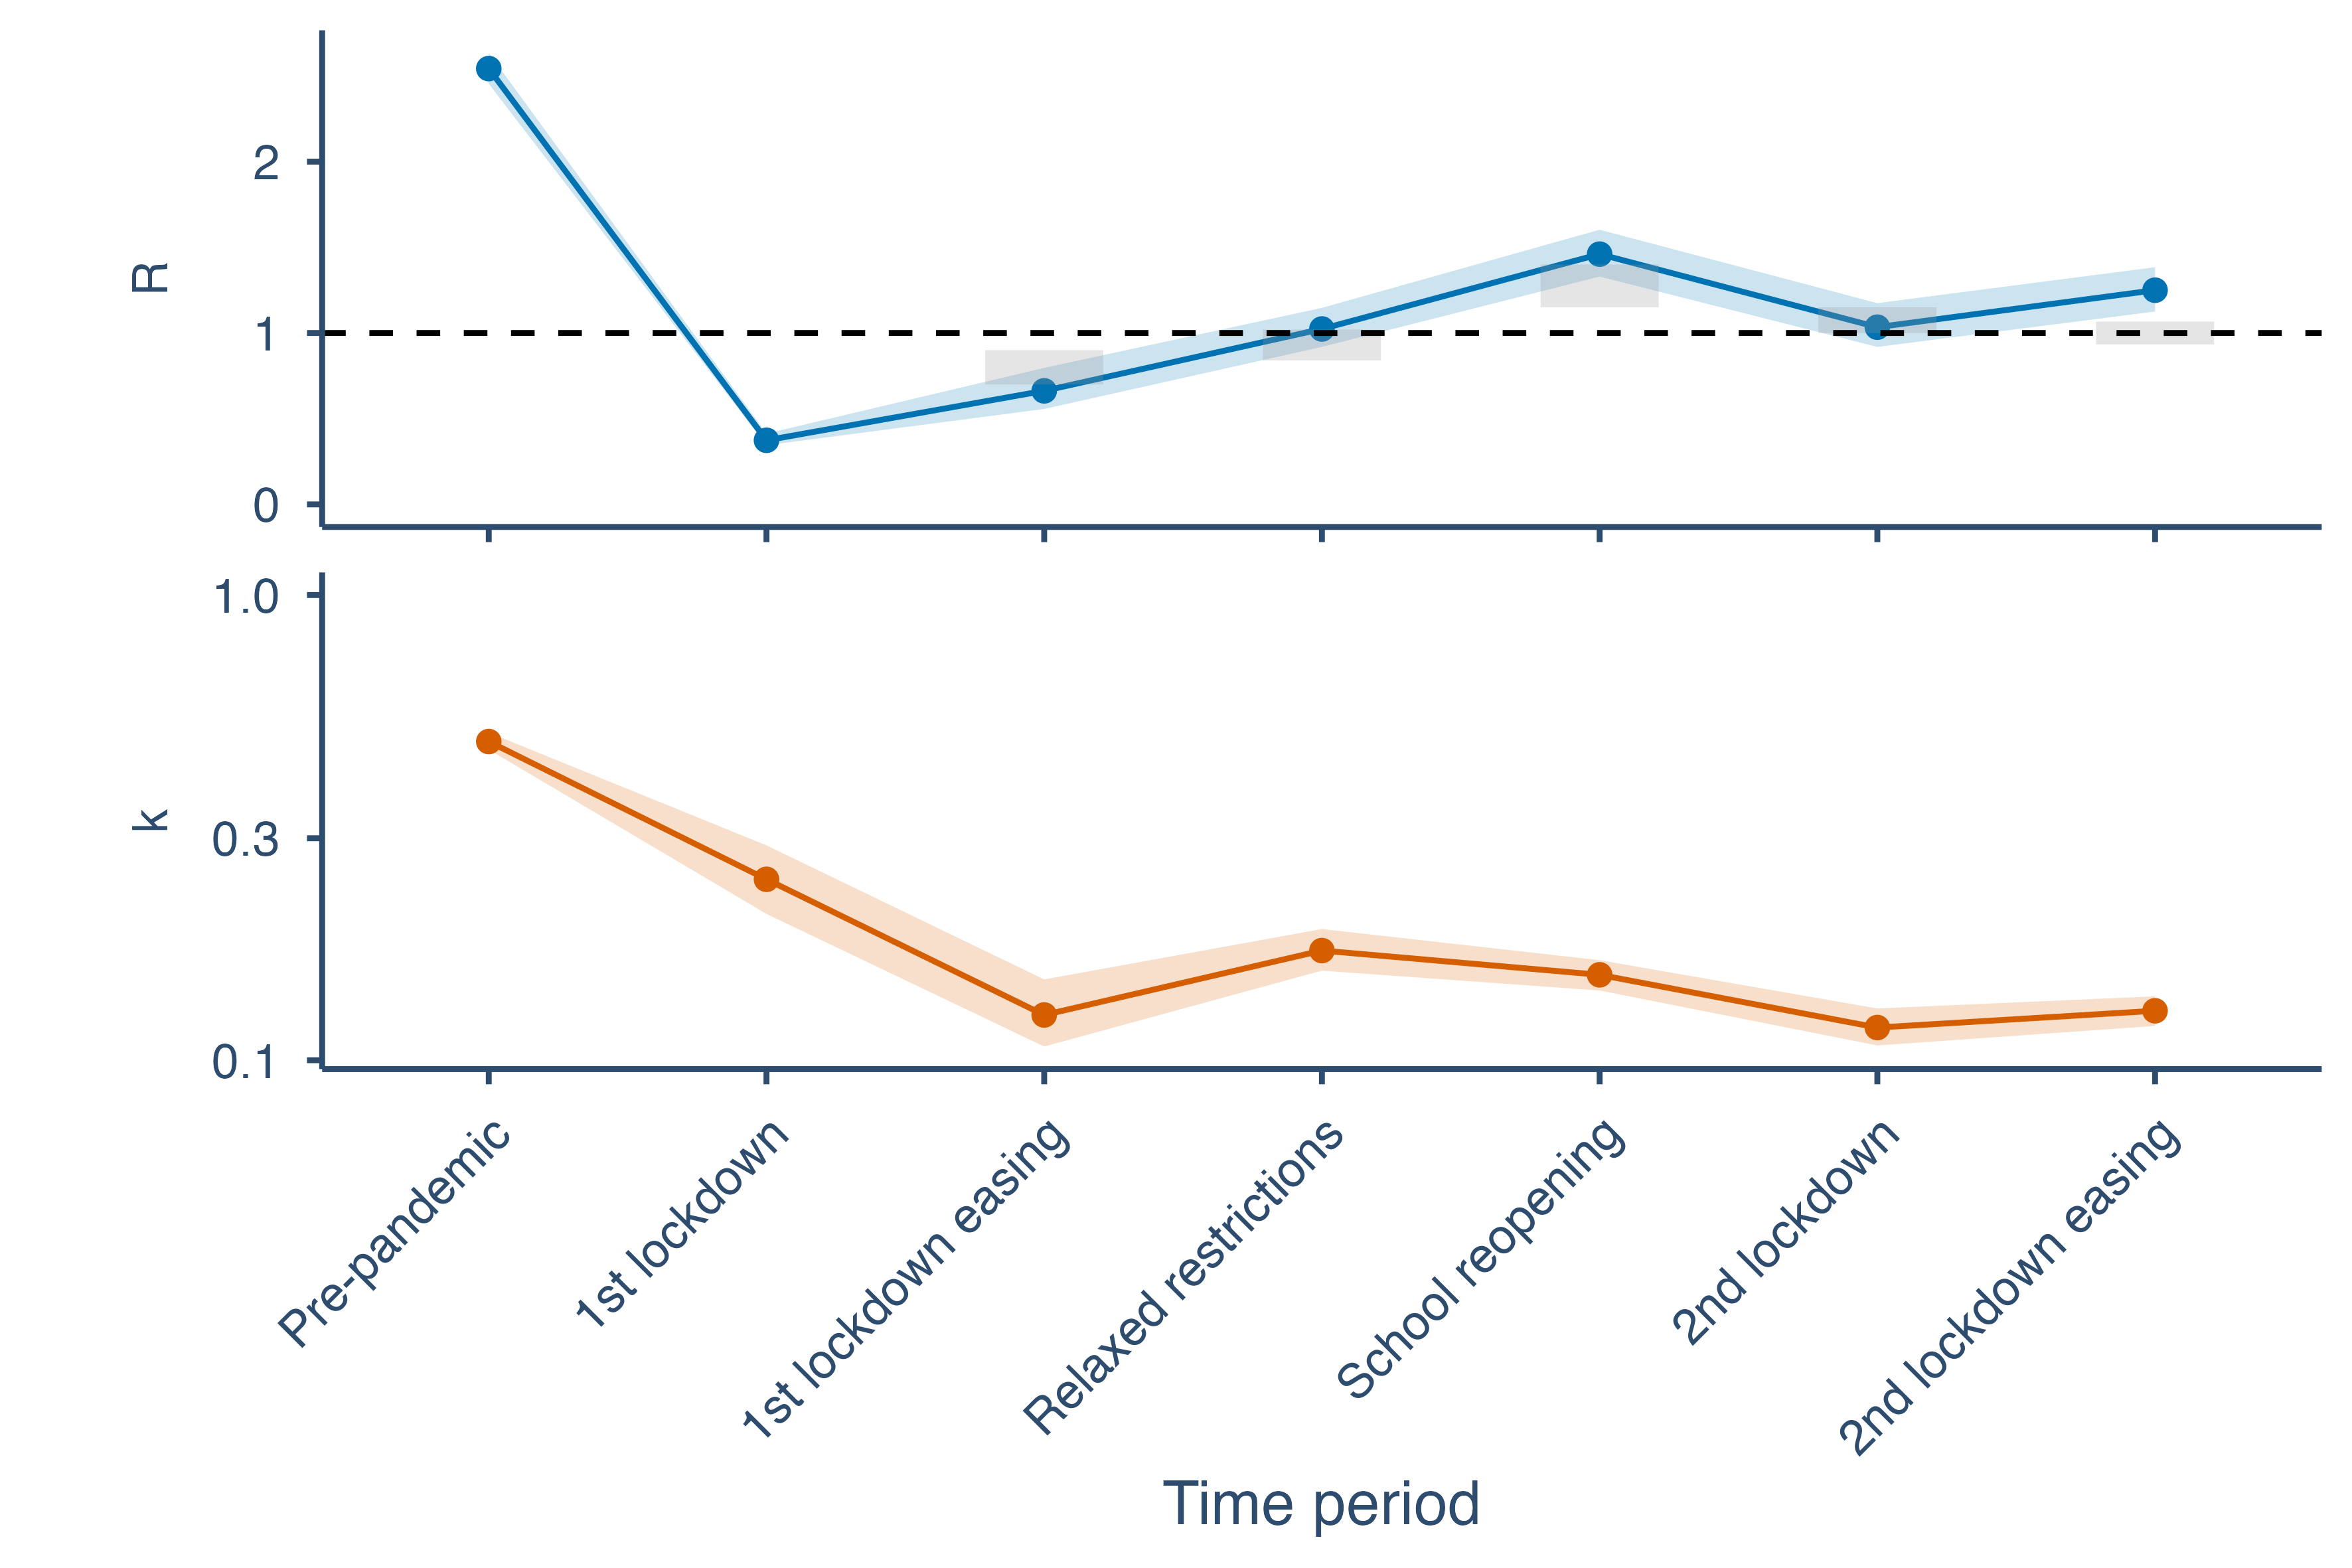
\includegraphics[width=1\linewidth,height=\textheight,keepaspectratio]{../results/manuscript_figures/fig4_rk.png}

}

\caption{\label{fig-rk}Estimates of the mean and dispersion of negative
binomial distributions fitted to simulated secondary infection
distributions by time period in 2020. The dispersion parameter \(k\)
gives an indication of the variation in the secondary infection
distribution, with smaller values corresponding to greater variation and
values less than 1 corresponding to very large variation. Grey boxes in
the \(R\) plot show the average upper and lower bounds (90\% confidence
interval) of the consensus estimates published by the Scientific
Pandemic Influenza group on Modelling in the UK for the specified time
periods. Shaded bands show 95\% bootstrap confidence intervals for the
\(R\) and \(k\) estimates.}

\end{figure}%

\subsubsection{Contribution to heterogeneity in secondary infections due
to variation in contact rates and viral load
progression}\label{contribution-to-heterogeneity-in-secondary-infections-due-to-variation-in-contact-rates-and-viral-load-progression}

If both contact rates and viral load trajectories are treated as
homogeneous, with Poisson-distributed contacts and no variation in viral
load trajectory between individuals, then the secondary infection
distribution is approximately Poisson with equal mean and variance,
corresponding to very large values of \(k\). If contacts are Poisson
distributed but viral load trajectories are allowed to vary between
individuals, \(k\) is 1.5 -- 1.9. If viral load is fixed at the median
trajectory, but contacts are overdispersed, values of \(k\) are lower
(0.11 -- 0.74) and approximately equal to that of overdispersed contacts
and variable viral load trajectories (0.11 -- 0.51), indicating that
overdispersion in numbers of daily contacts, as the denominator in the
infection process, contributes more to superspreading, meaning
overdispersion in the secondary infection distribution, than variable
viral load trajectories (Figure~\ref{fig-heterogen}). The two
overdispersed-contact scenarios, equal and variable viral load, differ
only pre-pandemic (\(k\) = 0.74 versus 0.51). This is due to individuals
in the upper tail of infectiousness generating disproportionately many
secondary infections when contacts are plentiful, as a result of the
right-skewed area-under-the-curve distribution, exceeding an 73-fold
range (Figure~\ref{fig-vl}D). During restriction periods this difference
disappears, as compressed contact rates create a ceiling on secondary
cases regardless of viral load, and the proportion infecting zero others
and more than ten others converges across the two scenarios from the
first lockdown onwards (Figure~\ref{fig-heterogen}). In the sensitivity
analysis with greater variation in individuals' viral load trajectories,
with double the standard deviation in the viral load trajectory
parameters, the \(k\) estimates for the scenario with Poisson contacts
(0.76 -- 0.92) and variable viral loads were closer to those for
overdispersed contacts and variable viral loads (0.08 -- 0.33), but
still higher (Figure S8). The finding that contact heterogeneity plays a
greater role in overdispersion in secondary infections than viral load
heterogeneity therefore appears to be robust to much greater variation
in peak viral load and duration of viral shedding than found in the
cohort in Kissler et al. \citep{kissler2021}.

\begin{figure}

\centering{

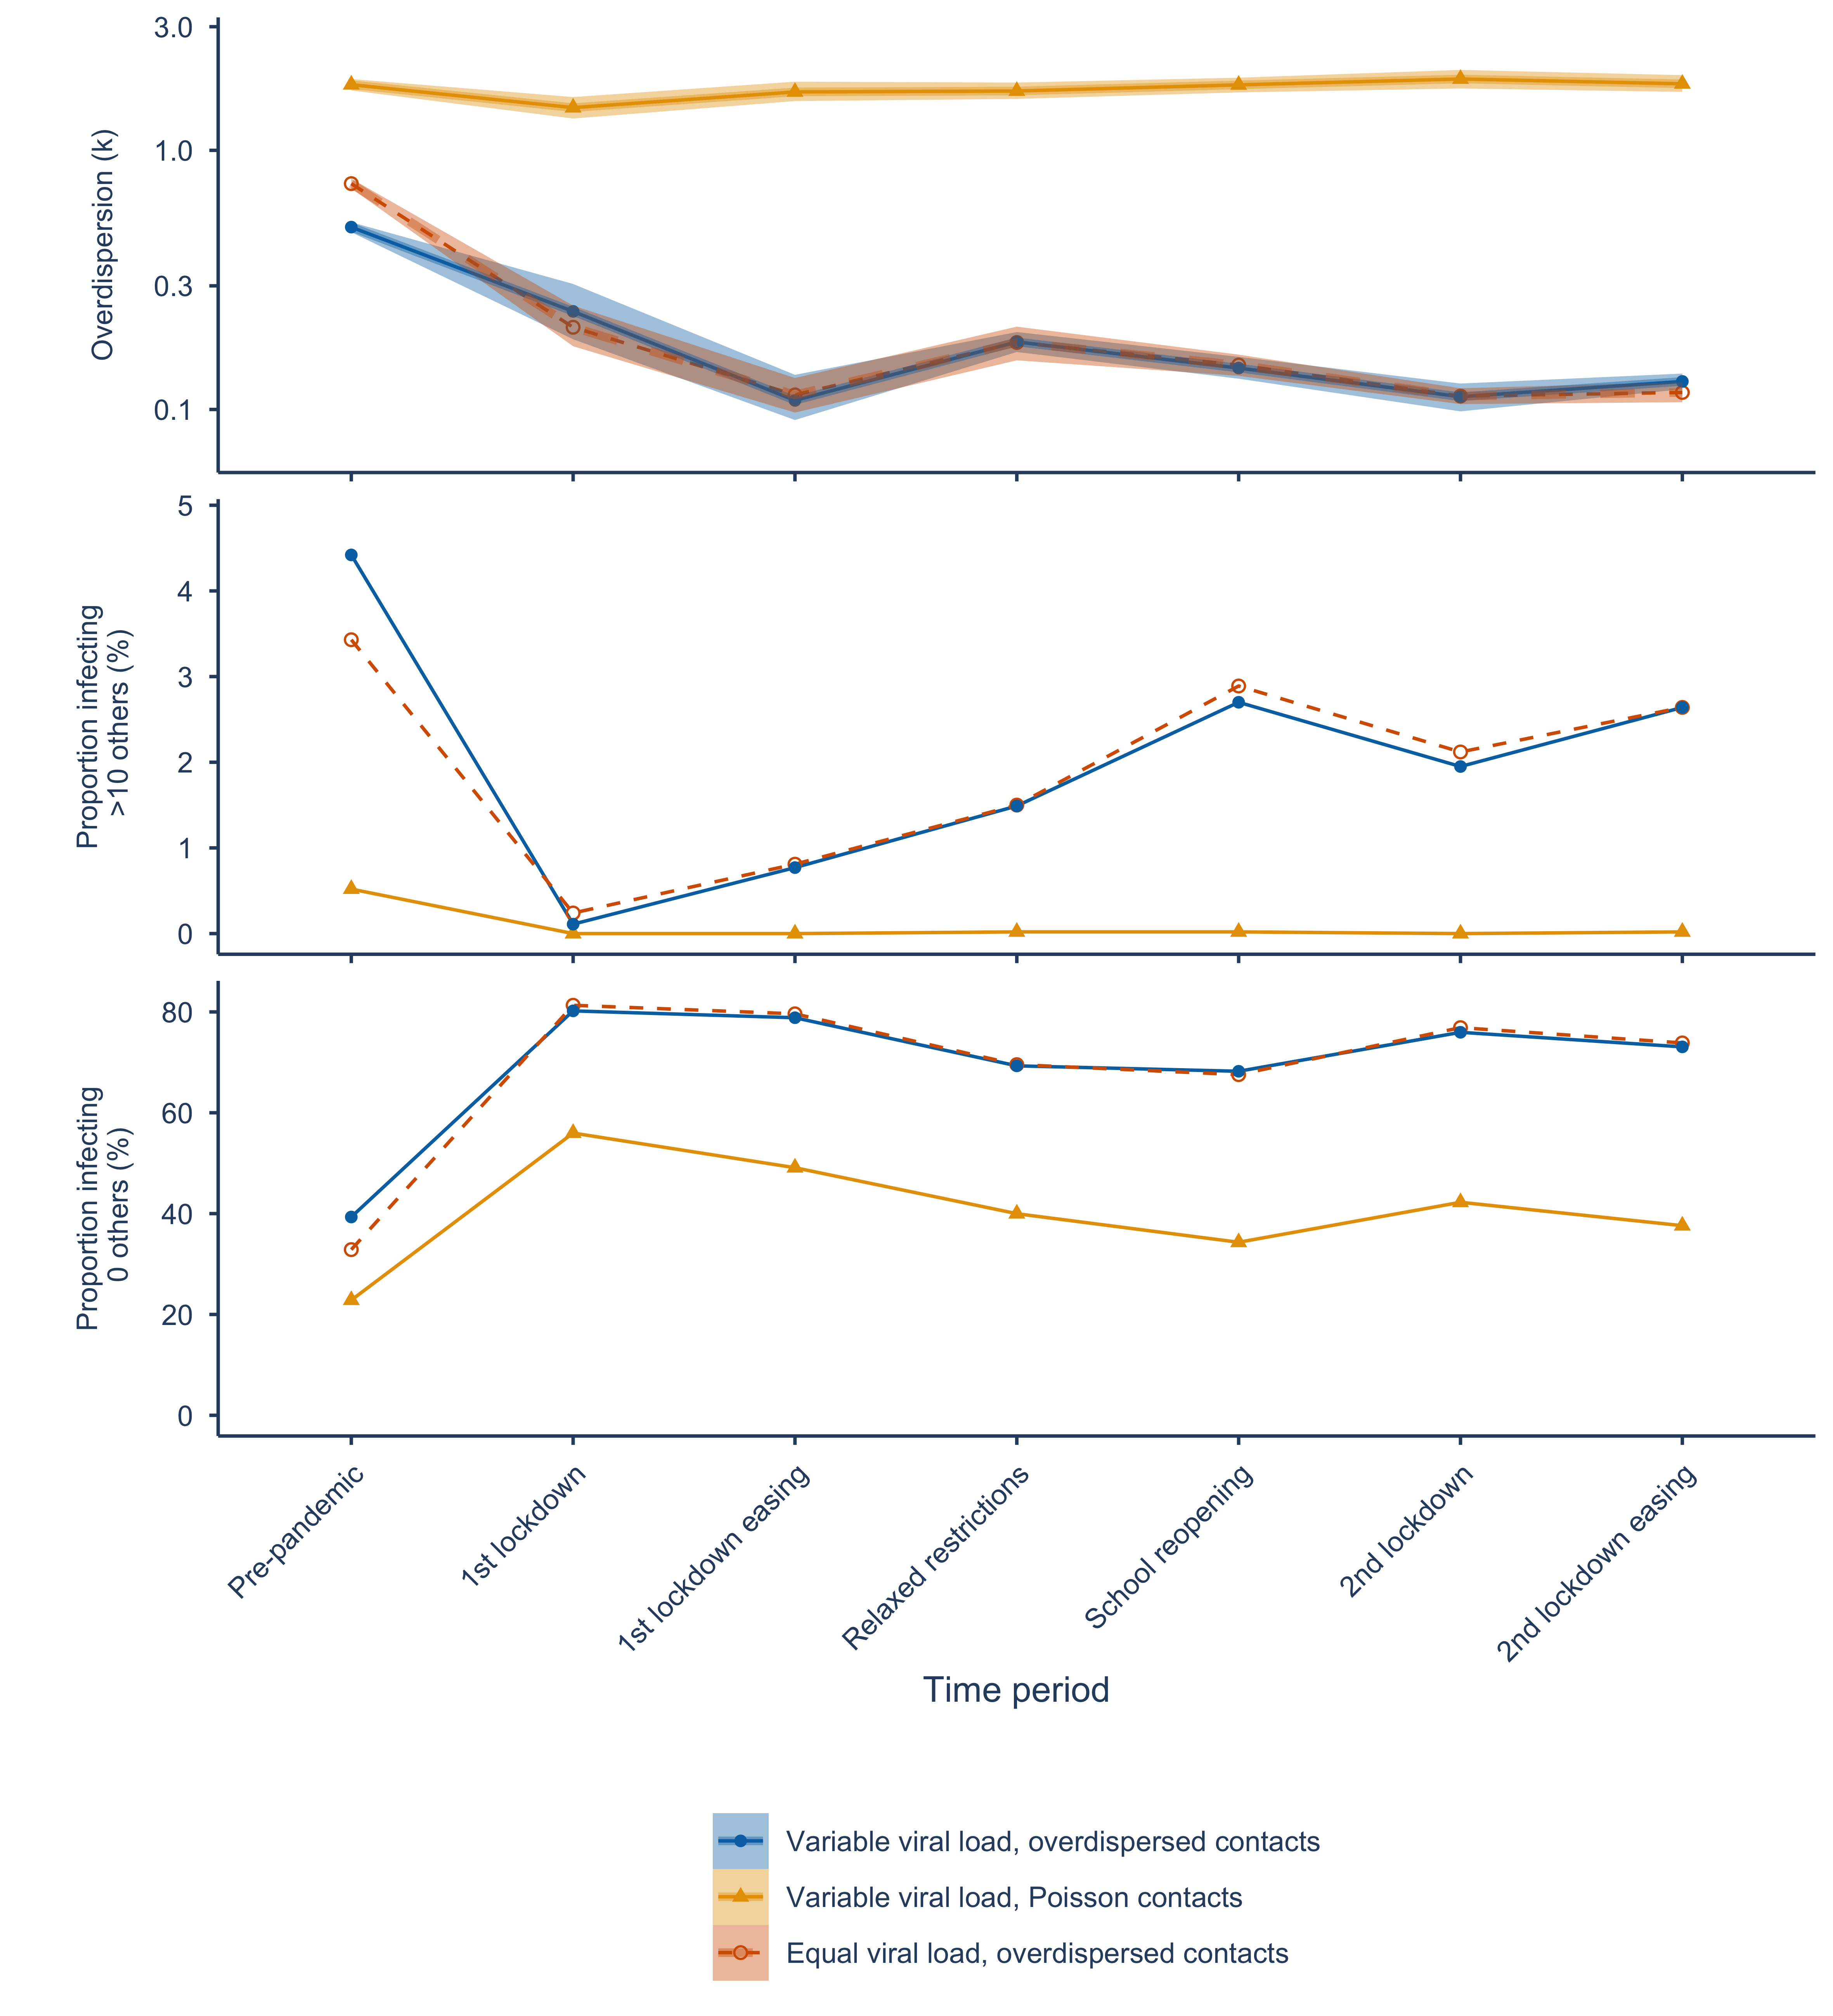
\includegraphics[width=1\linewidth,height=\textheight,keepaspectratio]{../results/manuscript_figures/fig5_heterogen.png}

}

\caption{\label{fig-heterogen}Estimates of the dispersion of negative
binomial distributions fitted to secondary infection distributions by
period, with different combinations of homogeneous and heterogeneous
contact rates and viral load trajectories, along with the proportion of
individuals infecting zero others and more than ten others. The
dispersion parameter \(k\) gives an indication of the variation in
numbers of secondary infections, with smaller values corresponding to
greater variation and values less than 1 corresponding to very large
variation. Values of \(k\) for equal viral load and equal contacts are
not shown because they are very large, meaning the numbers of secondary
infections are approximately Poisson distributed. Shaded bands show 95\%
bootstrap confidence intervals. The sensitivity analysis with greater
variation in viral loads is shown in Figure S8.}

\end{figure}%

\subsubsection{Impact of rapid testing (regular testing vs.~pre-event
testing)}\label{impact-of-rapid-testing-regular-testing-vs.-pre-event-testing}

For pre-pandemic levels of contacts, uptake of regular LFT testing must
exceed 70\% to reduce \(R\) below 1 if testing daily and must be above
80\% if testing every 3 days, but even 100\% uptake will not reduce
\(R\) below 1 if testing weekly (Figure~\ref{fig-testing}A). For
lockdown levels of contacts, testing does not appreciably reduce \(R\)
below its already low level. For contact rates equivalent to those under
relaxed restrictions with schools open, testing every 3 days will reduce
\(R\) below 1 if uptake exceeds 70\% (Figure~\ref{fig-testing}A).
Pre-event testing acts similarly, with high uptake (\textgreater{} 90\%)
and testing for events with more than 10 others necessary to reduce
\(R\) below 1 for pre-pandemic levels of contact, but only testing when
attending events with more than 20 others and 60\% adherence required
during relaxed restrictions with schools open
(Figure~\ref{fig-testing}B). Both regular testing and pre-event testing
reduce the rate of superspreading as defined as the proportion of
individuals infecting over 10 others. However, there is also an increase
in the proportion of individuals that infect no one. In some cases, this
results in a decrease in \(k\) (greater overdispersion in the secondary
infection distribution) (Figure~\ref{fig-testing} ). From the
sensitivity analysis comparing the impact of regular testing with and
without overdispersion in contacts (Figure S9), we can see that ignoring
overdispersion in contacts reduces the estimated impact of testing in
terms of reducing \(R\) and decreasing the proportion of superspreading
events. This demonstrates the importance of accounting for contact
overdispersion when estimating the impact of interventions on secondary
infections.

\begin{figure}

\centering{

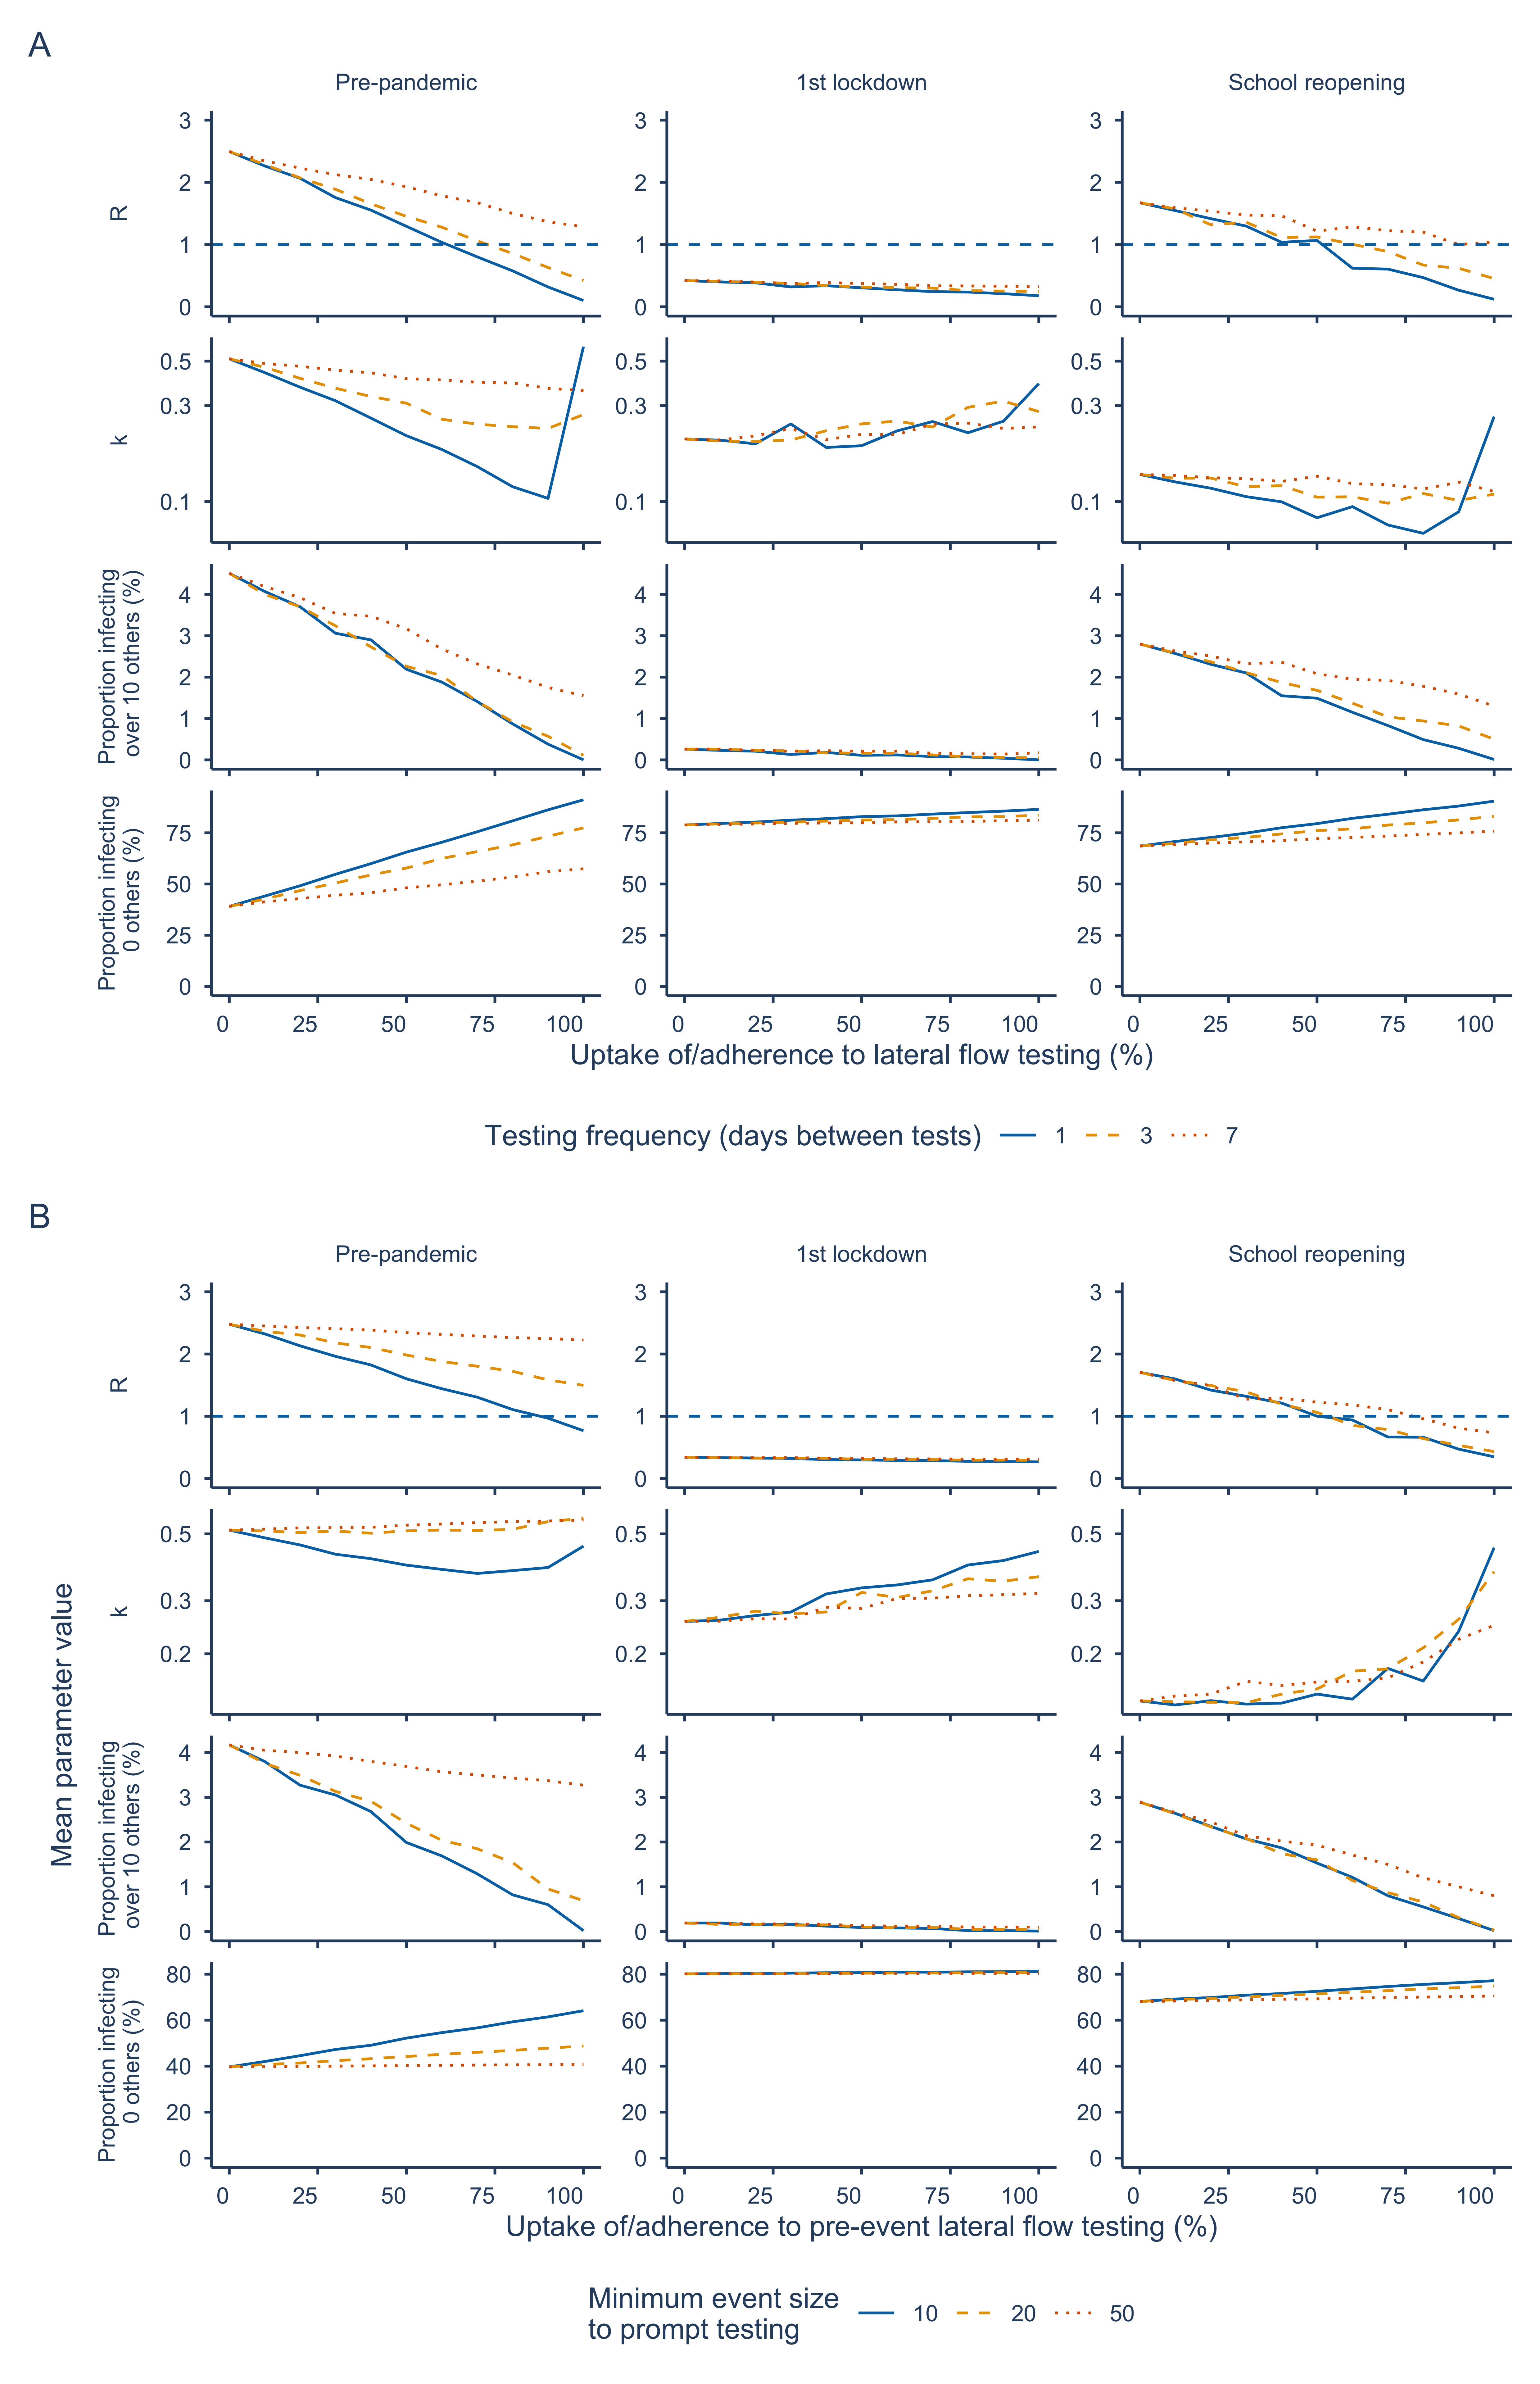
\includegraphics[width=1\linewidth,height=\textheight,keepaspectratio]{../results/manuscript_figures/fig6_testing.png}

}

\caption{\label{fig-testing}Effect of regular and pre-event lateral flow
testing on \(R\), \(k\), and the proportion infecting over 10 or 0
others for varying levels of uptake or adherence (horizontal axes) and
background contact rates (columns). A. Regular testing. B. Pre-event
testing.}

\end{figure}%

\subsection{Discussion}\label{discussion}

We have estimated the secondary infection distribution for SARS-CoV-2
over the course of the pandemic in the UK in 2020 using a stochastic
model incorporating viral load trajectories and reported daily contacts.
Our estimates of the mean number of secondary infections are consistent
with contemporaneous estimates (Figure~\ref{fig-rk}). Daily contact
rates became both lower on average, from 11.5 per day to 4.7 per day,
and more overdispersed during the pandemic in the UK in 2020 as some
individuals maintained high contact rates, such as essential workers,
while others had their number of daily contacts reduced to zero, such as
those working from home. This drove a decrease in the mean number of
secondary infections per infected individual, the reproduction number,
but an increase in the dispersion in the number of secondary infections.
Our estimates of the degree of overdispersion in the secondary infection
distribution are similar to those reported by other authors, which are
mostly between 0.3 and 0.6 \citep{lau2020, kremer2021}, though lower
estimates of around 0.1 have been reported from outbreak cluster size
data \citep{endo2020}.

Our analysis shows that changes in the mean and overdispersion of daily
numbers of contacts over time (Figure~\ref{fig-contacts}C) can be used
to estimate dynamic shifts in the mean and overdispersion of the
reproduction number (Figure~\ref{fig-rk}). This motivates collecting
contact data during epidemics, as contact overdispersion could provide a
potential indicator of superspreading risk in real-time, along with the
effective reproduction number. Changes in contact overdispersion would
indicate when and where the population is at risk of superspreading
events, and enable implementation of targeted, rather than blanket,
restrictions on contact levels to limit outbreaks. However, ground-truth
data on secondary infection distributions, e.g.~from contact tracing
studies, would first be required to validate estimates of the mean and
overdispersion of the secondary infection distribution.

Contact heterogeneity was found to contribute more to superspreading
than heterogeneity in viral load, as the number of contacts an
individual makes places an upper limit on the number of people they can
infect, and, despite some individuals having much higher infectious
potential than others, most infected individuals pass through a high
viral load period, with 68\% having a peak culture probability greater
than 0.6 and 53\% greater than 0.8. Viral load heterogeneity does still
contribute significantly to heterogeneity in transmission since viral
load varies by orders of magnitude over time within individuals and
between individuals (Figure~\ref{fig-heterogen}). This indicates that
superspreading is more a result of between-person contact variability
and within-person infectiousness variability than between-person
infectiousness variability. Hence if reductions in contact rates can be
targeted specifically at individuals ahead of or during their window of
high infectivity, for example by encouraging contacts of cases to
undergo regular self-testing and self-isolation upon a positive rapid
test result \citep{quilty2021}, then this may result in reductions in
transmission while minimising the burden of quarantine. Other studies
investigating the superspreading nature of SARS-CoV-2 have come to
similar conclusions
\citep{susswein2020, ke2022, goyal2021, sun2021, ke2021pnas, hart2023}.
However, as far as we are aware our study is the first to estimate the
relative roles of contact and viral load heterogeneity and the impact of
changes in contact heterogeneity using real-world contact distributions
from before and during the pandemic and data on viral load trajectories
and infectiousness \citep{pickering2021}. Our use of reported
heterogeneity in viral load trajectories \citep{kissler2021} also
contributes to a wider estimated distribution for the number of days
individuals are likely infectious, which closely matches empirical daily
sampling \citep{ke2022} and human challenge studies
\citep{killingley2022}. Our approach of using culture positivity as a
direct virological proxy for infectiousness is complementary to that of
Marc et al. \citep{marc2021}, who inferred the viral-load-infectiousness
relationship from observed transmission outcomes and similarly found
that viral load alone does not fully explain transmission heterogeneity,
with a residual random effect standard deviation of 85\%. Consistent
with our findings, Kendall et al. \citep{kendall2024} found that contact
rates explained more daily variability in \(R(t)\) than per-contact
transmissibility (46\% versus 30\%) using NHS COVID-19 app data that
tracked CoMix closely; Ferretti et al. \citep{ferretti2024} similarly
found that contact duration drove transmission risk more than proximity,
supporting the use of duration-weighted contacts in our model.

Like others \citep{ke2022, hart2023, middleton2024}, we hypothesised
that lateral flow testing, by detecting individuals with high viral
loads when they were most infectious, would reduce transmission through
reducing the potential for superspreading. This manifested as a decrease
in the proportion infecting over 10 others and a substantial increase in
the proportion infecting zero others. This, perhaps counter-intuitively,
resulted in a decrease in \(k\) in some cases, as the relative increase
in those infecting zero others exceeded the decrease in those infecting
many others, here defined as over 10 others. Hence, assessment of
superspreading solely via the metric of the overdispersion parameter
\(k\) may conceal changes in both the upper and lower tail of the
secondary infection distribution. Both regular testing and pre-event
testing were effective in reducing \(R\) given high enough frequency or
a low enough event size threshold, respectively, as long as uptake or
adherence was high. Testing had the highest relative impact on
transmission when contact rates were high, for example at pre-pandemic
levels, as there were more potentially preventable exposures, meaning
rapid testing could reduce \(R\) below the growth threshold of 1 while
otherwise maintaining relatively normal contact rates. In contrast,
testing during lockdown would have less impact as \(R\) was already
below 1. Having everyone in the population test every 3 days would bring
\(R\) below 1 and be approximately equivalent in terms of impact on
secondary infections to having people test only before events of minimum
size 10 for pre-pandemic contact levels. This indicates that rapid
testing could be an effective, minimally disruptive intervention to
reduce transmission if uptake or adherence could be maximised through
incentivising use. Our findings align with those of Ke et al.
\citep{ke2022}, who estimated using a within-host model of infection
that daily antigen testing could reduce infectiousness by 85\% but that
impact reduced significantly with decreasing testing frequency. However,
our analysis goes further by estimating the impact of different rapid
testing frequencies on the reproduction number accounting for the full
distribution of daily contacts. Hart et al. \citep{hart2023} similarly
found that daily lateral flow testing could significantly reduce numbers
of secondary infections, preventing around 70\% of infections assuming
complete isolation of infected individuals following detection, although
they used a full multiscale model of within-host dynamics and
transmission and focused on the Omicron variant, for which the
effectiveness of testing may be different due to differences in
within-host dynamics and pre-existing immunity.

In their analysis of the CoMix data, Gimma et al. \citep{gimma2022}
found that school-aged children consistently had higher numbers of
contacts across both lockdowns and periods of relaxed restrictions than
working-age adults, who in turn had higher numbers of contacts than
older adults (60+ years). Contact levels also varied with employment
status, with part-time-employed participants having more contacts than
full-time or self-employed participants. Another analysis of the CoMix
data that focused on individuals with high numbers of contacts
\citep{chapman2021} identified that most reports of high numbers of
contacts came from work and school settings and tended to be reported by
participants in certain professions (teaching, retail, administration,
construction, medicine, social work, hospitality). Some of this work is
considered essential, and keeping schools open where possible is a high
priority, so opportunities for reducing these contacts may be limited.
This highlights the potential value of regular rapid testing as a way of
preventing superspreading even when some individuals have many contacts.

Our analysis has some limitations. The CoMix contact survey was designed
to be comparable to previous contact surveys in the UK, namely the BBC
Pandemic \citep{klepac2018, klepac2020, kucharski2020} and POLYMOD
\citep{mossong2008} surveys. However, previous surveys required
participants to list contacts individually to include other information
such as contact age, sex, and occupation, meaning that it was difficult
to include mass contacts such as those made at a large gathering, thus
truncating the true contact distribution (Figure~\ref{fig-contacts}B).
From 18 May 2020 the CoMix survey introduced the option to record mass
contacts as a count rather than listing each contactee in a separate
entry. This means pre-pandemic and early-pandemic contact distributions
are not directly comparable to those conducted later. However, we
conducted a sensitivity analysis to check how this could impact our
estimates of numbers of secondary infections, by imputing a heavier tail
for the BBC Pandemic contact distribution based on the tails of the
contact distributions during periods of relaxed restrictions in the
CoMix survey, and observed only a small increase in \(R_0\) and a small
reduction in \(k\). Additionally, variation between participants in how
direct contacts are interpreted and reported could contribute to
artificial overdispersion in the contact distribution and hence in our
estimates of secondary infection overdispersion. Another limitation of
the BBC Pandemic contact data is that working-age adults were
overrepresented among the participants, while children under 13 years
were excluded (Figure S3). It is possible that this may have led to some
bias in the reported contact distributions. However, the similarity of
contact patterns observed in the BBC Pandemic and UK POLYMOD datasets
\citep{klepac2020} suggests that the BBC Pandemic data is broadly
representative of pre-pandemic contact patterns in the whole UK
population.

We used data on viral loads over time from a detailed study of
individuals in the National Basketball Association cohort in Kissler et
al. \citep{kissler2021}, which is unlikely to be representative of the
full variation in viral load trajectories in the general population,
since the cohort consisted mostly of young, healthy, male professional
athletes. Our analysis could therefore underestimate the variability in
secondary infections due to variability in viral load with factors such
as age, for which there is some evidence of an effect on infectiousness
\citep{ke2022}, co-morbidities, and sex. In particular, the NBA cohort
does not include individuals with very long infections. Ghafari et al.
\citep{ghafari2024}, for instance, found that some individuals in the
Office for National Statistics COVID-19 Infection Survey in the UK had
persistent infections lasting more than 60 days. However, they
constituted only 0.1 to 0.5\% of all infections, with PCR-derived viral
loads around 100-fold lower than at symptom onset, substantially
reducing their transmission potential. Furthermore, PCR measurements
were only taken from ONS infection survey participants weekly for a
month and then monthly up to a year, whereas measurements were near
daily in the NBA cohort and crucially captured the early stage of
infection, and therefore permit much higher resolution modelling of
onward transmission. We conducted a sensitivity analysis with much
greater variation in viral load trajectories to account for greater
variation in the general population and found that it did not
qualitatively change our conclusion that contact heterogeneity remains
the primary driver of heterogeneity in transmission.

We assume that the probability of shedding infectious virus is equal to
the probability of culturing virus, but the exact relationship between
viral culture positivity and infectiousness is not known
\citep{puhach2023}, so our results must be interpreted with this
limitation in mind. Furthermore, the specific proportions of infectious
individuals we report depend on the fitted logistic dose-response curve
between viral load and culture probability; alternative functional forms
would yield different estimates. A structural asymmetry in our
comparison is that contact heterogeneity is measured directly from
survey data, whereas infectiousness heterogeneity is captured only via
viral load as a proxy. Sources of between-individual variation in
infectiousness that are decoupled from within-host viral dynamics, such
as variation in respiratory droplet production, speaking volume, or
interpersonal distance preferences, are not captured, and if substantial
would increase the true contribution of infectiousness heterogeneity
relative to our estimates. We partially address this by drawing the
logistic regression coefficients linking viral load to infectiousness
for each individual from the estimated covariance distribution, and by
examining robustness in a sensitivity analysis with twice the standard
deviation in viral load trajectory parameters (Figure S8); however,
these measures do not capture variation in transmission efficiency that
is entirely independent of viral load. We also do not account for
correlation of the timing of peak viral load and infectiousness with
symptom onset and intensity \citep{marks2021}, which may affect contact
rates and numbers of secondary infections \citep{marc2021}.

We focus on an index case and their infections in one other generation,
which may underestimate second-order effects that considering a full
contact network structure would capture \citep{ke2022}. For instance, we
would expect individuals that acquire infection to typically have higher
contact rates than the average member of the population, since having
more contacts increases acquisition risk, and therefore to infect more
individuals. However, incorporating this effect would require additional
assumptions about how acquisition risk scales with contact number and
network structure that we do not have the data to support. We do not
consider other interventions that may have an additional impact on
\(R\), such as vaccination, contact tracing, or self-isolation upon
symptom onset. We also do not consider the impact of variants with
increased transmissibility, and hence limit our analysis to 2020 before
the widespread emergence of variants of concern such as Alpha, Delta,
and Omicron.

We assumed within-household contacts for each individual were the same
each day, and sampled daily non-household contacts from repeat responses
for the same survey participant, which may underestimate variation in
overall daily contact rates and hence infection potential of specific
individuals. We assume that self-isolating individuals are unable to
fully self-isolate from their household members as reported by the
majority of those surveyed by the ONS in England in April 2021
\citep{ons2021}; further decreases in \(R\) may be possible if
self-isolating individuals isolate themselves from household members.

There is some evidence that heterogeneity in secondary infections has
changed as new SARS-CoV-2 variants of concern have emerged and
population immunity has increased. Studies examining heterogeneity in
SARS-CoV-2 transmission over time in Japan and Europe have found that
overdispersion remained after the emergence of Alpha, Delta, and
Omicron, with \(k\) generally being below 0.5 but varying somewhat
across waves and being higher, that is, less overdispersed transmission,
during the Omicron wave \citep{ko2023, hodcroft2025}. Meta-analyses of
literature estimates of \(k\) have shown a wide range of estimates
across settings, clusters and variants, but no clear trend in \(k\) over
time \citep{du2022, wegehaupt2023}, though some studies suggested slight
increases in \(k\) with the emergence of Delta. A modelling study has
suggested that non-pharmaceutical interventions such as lockdowns have
imposed selective pressure on SARS-CoV-2 towards more homogeneous
transmission, corresponding to higher \(k\) \citep{nielsen2022}.
Together, these studies suggest that while overdispersion may be
weakening with widespread immunity and new variants of concern, it
remains a feature of SARS-CoV-2 transmission.

Thus, while our analysis is restricted to 2020, our findings are still
relevant in the current era of endemic COVID-19 and to other pathogens
that exhibit heterogeneous transmission, including other SARS
coronaviruses, Ebola, measles, influenza, RSV, and adenoviruses
\citep{goyal2021, leung2021, lloydsmith2005}. Moreover, the question of
the relative contribution of variation in numbers of contacts and
variation in infectiousness to heterogeneity in transmission is a
universal one for infectious diseases. By demonstrating that
superspreading potential is closely linked to the overdispersion of
social contacts and the timing of peak infectiousness, we have shown the
importance of monitoring not only the mean effective reproduction number
but also its variability. Measurement of contact distributions thus
offers a real-time surveillance tool for identifying superspreading
risk, supporting pandemic preparedness through enabling targeted
interventions against emerging pathogens. The modelling framework is
generalisable: provided densely sampled pathogen load trajectories and
pathogen-specific culture or test sensitivity data are available to
characterise infectiousness, and a contact survey with duration
information is available to characterise the contact distribution, the
same approach can be applied to estimate heterogeneity in the secondary
infection distribution for other pathogens.

Our results suggest superspreading for SARS-CoV-2 can be best explained
as a random sample from the tail of the contact and shedding
distribution: it occurs when an infected individual makes a high number
of contacts during a highly infectious period lasting approximately 2
days on average, with the majority of infected individuals being
sufficiently infectious, 68\% with a peak culture probability over 0.6
and 53\% over 0.8, for at least one day to be capable of causing a
superspreading event, given they make a high number of contacts. Changes
in the number of contacts observed throughout the pandemic in the CoMix
contact survey were able to explain changes in the reproduction number,
with contact rates becoming more heterogeneous during the pandemic given
lockdowns and changes in working practices. For future pandemics,
regular or pre-event lateral flow testing may be an efficient way to
target individuals when most infectious and hence minimise the burden of
non-pharmaceutical interventions while maximising reduction in
transmission rates, provided uptake is moderate to high.

\subsection{Supporting Information}\label{supporting-information}

\paragraph*{Figure S1}
\label{fig-s1}
{\textbf{Distribution of the duration of contact for household and
out-of-household contacts from the CoMix contact survey in the UK.}}

\paragraph*{Figure S2}
\label{fig-s2}
{\textbf{Correlation between number of contacts and mean contact
duration for CoMix survey participants from March 2020 to May 2021.}}

\paragraph*{Figure S3}
\label{fig-s3}
{\textbf{Age distribution of participants in the BBC Pandemic
(Pre-pandemic) contact survey and each of the nine time periods from the
CoMix contact survey from March 2020 to May 2021 relative to the
mid-2020 UK age distribution \citep{ons2022}.}}

\paragraph*{Figure S4}
\label{fig-s4}
{\textbf{Contact distributions for three indicative timepoints before
and during the pandemic in the UK with an imputed heavier tail in the
Pre-pandemic (BBC Pandemic) contact distribution (cf.~Figure 2B).}} The
heavier tail was imputed from the tails of contact distributions during
periods of relaxed restrictions in the CoMix survey. We conducted a
sensitivity analysis with this distribution to determine the effect of
the heavier tail on \(R_0\) and \(k\).

\paragraph*{Figure S5}
\label{fig-s5}
{\textbf{Distribution of the number of reported daily contacts for all
time periods before (BBC Pandemic contact survey) and during (CoMix
contact survey) the pandemic in the UK between March 2020 and May
2021.}}

\paragraph*{Figure S6}
\label{fig-s6}
{\textbf{Contact distributions by age and gender across the nine time
periods from the CoMix contact survey from March 2020 to May 2021.}}

\paragraph*{Figure S7}
\label{fig-s7}
{\textbf{Comparison of viral load trajectories and infectivity for the
sensitivity analysis with double the standard deviation in viral load
trajectory parameters and those used in the main analysis.}} A.
Individual-level viral load trajectories. B. Logistic model for
probability of culturing virus given a certain viral load. C. Relative
infectivity over time. D. Area under the infectivity curve, in arbitrary
units. E. Distribution of the number of days for which individuals were
infectious. Solid lines in A and C represent median viral load and
infectivity trajectories. The dashed line in A and B represents the RNA
copies per ml required for a 50\% probability of culturing virus or
infectiousness. The shaded band in B represents the uncertainty in the
probability of culturing virus given a certain viral load from the
fitted logistic regression model from Pickering et al.

\paragraph*{Figure S8}
\label{fig-s8}
{\textbf{Sensitivity of estimates of dispersion of the secondary
infection distribution in different time periods to the degree of
variation in viral load trajectories.}} Left: standard deviation in
distributions for viral load trajectory parameters from Kissler et
al.~Right: standard deviation of viral load parameters doubled.

\paragraph*{Figure S9}
\label{fig-s9}
{\textbf{Comparison of the impact of regular lateral flow testing on
\(R\), \(k\), and the proportion infecting over 10 or 0 others with
Poisson-distributed contacts and overdispersed contacts, for varying
levels of uptake or adherence and background contact rates.}}

\paragraph*{Table S1}
\label{tbl-s1}
{\textbf{Sensitivity analysis of the effect on \(R\) and \(k\) when
imputing a heavier tail of the contact distribution for the pre-pandemic
BBC Pandemic contact survey, which lacked the ability to record raw
counts of high numbers of contacts.}}

\paragraph*{Table S2}
\label{tbl-s2}
{\textbf{Sensitivity analysis of the effect on the mean and dispersion
in contact rates comparing a negative binomial distribution to a
zero-inflated negative binomial distribution.}}

\subsection{References}\label{references}

\renewcommand{\bibsection}{}
\bibliography{references.bib}


\nolinenumbers


\end{document}
